%+----------------------------------------------------------+
%| SLIDES: Construction and Reduction of the L-infinity Algebra of Observables
%|         Associated with a BV-Module
%| Contents: - 60 minutes (estimated duration ~2.5 minutes per slide, ~24 slides)
%|
%| Author: Antonio Miti
%| Event: ARTS — Algebra and Representation Theory Seminar
%| Place: Università di Roma  "Tor Vergata "
%| Date: 21/10/2025
%| Link: https://www.mat.uniroma2.it/~ricerca/algebr/page-AREA_files/page-AREA-2_files/talks.html
%+----------------------------------------------------------+



%- HandOut Flag -----------------------------------------------------------------------------------------
	\newif\ifHandout
	\Handouttrue  %uncomment for the printable version
	%Handling of flags it is not preserved when passing to standalone-subfiles!


%- D0cum3nt ----------------------------------------------------------------------------------------------
\ifHandout
	\documentclass[handout,10pt]{beamer}   
	\setbeameroption{show notes} %print notes   
\else
	\documentclass[10pt]{beamer}
\fi


%- Packages ----------------------------------------------------------------------------------------------
\usepackage{custom-style}
\usepackage{math}

%- Bibliography (Biber) ----------------------------------------------------------------------------------
\usepackage[backend=biber,style=alphabetic,maxnames=2]{biblatex}
\bibliography{bibfile.bib}

%- L30's ----------------------------------------------------------------------------------------------
\usepackage{quiver} %https://q.uiver.app/ % Not in Miktex!
\usetikzlibrary{nfold}
\usetikzlibrary{decorations.pathmorphing} 
\renewcommand{\Ham}{\mathrm{Ham}}
\usepackage{enumitem}
\setlist{topsep=0pt, leftmargin=*,label=$\bullet$}


%--Beamer Style-----------------------------------------------------------------------------------------------
\usetheme{toninus}

\usetikzlibrary{backgrounds}
  \tikzset{
    invisible/.style={opacity=0},
    visible on/.style={alt=#1{}{invisible}},
    alt/.code args={<#1>#2#3}{%
      \alt<#1>{\pgfkeysalso{#2}}{\pgfkeysalso{#3}} % \pgfkeysalso doesn't change the path
    },
  }


%- T1tle P4g3 -------------------------------------------------------------------------------------------
\title{Construction and Reduction of the $L_\infty$ Algebra of Observables Associated with a BV-Module} 
\subtitle{\href{https://www.mat.uniroma2.it/~ricerca/algebr/page-AREA_files/page-AREA-2_files/talks.html}{- ARTS - Algebra and Representation Theory Seminar in Roma "Tor Vergata"}}
\author[AMM]{
	\href{https://www.antoniomiti.it/}{Antonio Michele Miti}
	{\small joint work w/ Leonid Ryvkin}
}
\institute[SUR]{
	Sapienza Università di Roma \\
	Rome, Italy 	\\
	\vspace{.5em}
  \begin{tabular}[h]{ccc}
      \href{https://www.mat.uniroma1.it/en}{
\includegraphics[width=6cm]{./Logos/Sur_logo}} & & 
      \href{https://civis3i.univ-amu.fr/en/civis3i-alliance-programme}{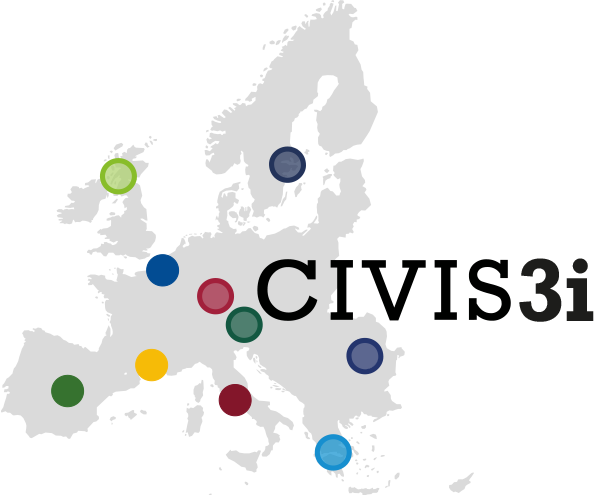
\includegraphics[width=3cm]{Logos/Civis_logo}}
  \end{tabular}    
}
\date[TorV25] % (optional, should be abbreviation of conference name)
{	
	{\vskip 1ex}
	Universit\'a di Roma - Tor Vergata, October 2025
}



%+----------------------------------------------------------+
%- D0cum3nt ------------------------------------------------+
%+----------------------------------------------------------+
\begin{document}
%+----------------------------------------------------------+

%----------------------------------------------------------------------------------+
\begin{frame}  % Alternative: \maketitle outside of frame
	\titlepage
	\ifHandout
		\tikz[overlay,remember picture]
		{
	    	%	\node at ($(current page.west)+(1.5,0)$) [rotate=90] {\Huge\textcolor{gray}{\today}};
	    	\node[        
	    		draw,
	    		shape border rotate=90,
			isosceles triangle,
			isosceles triangle apex angle=90,
			fill=yellow]
	        		at ($(current page.north east)-(1,1)$) [rotate=-45] {\textcolor{red}{Handout version}};
		}
	\fi
\end{frame}
\addtocounter{framenumber}{-1}
\note{
	%\textbf{\underline{OUTLINE}}:
	%\tableofcontents
	\textbf{Abstract:}
	\\
	\footnotesize
Multisymplectic manifolds generalize symplectic manifolds by carrying a closed, nondegenerate differential form of degree higher than 2. Such structures naturally arise in the geometric formulation of classical field theories.
Rogers (2010) showed that, just as a symplectic manifold yields a Poisson algebra of functions, an n-plectic manifold gives rise to an n-term Lie infinity algebra of observables.
Remarkably, his construction is purely algebraic and based only on Cartan calculus, suggesting that this higher “Poisson algebra” can be generalized beyond manifolds.
In this talk, we present such a generalization within the setting of Gerstenhaber algebras and Batalin–Vilkovisky (BV) modules, which provide an algebraic formulation of Cartan calculus relevant to noncommutative geometry.
This framework allows us to define Lie infinity algebras of observables in a fully algebraic way, without referring to an underlying manifold.
As an application, we address the reduction of multisymplectic observables in the presence of constraints or symmetries. Building on the work of Dippel, Esposito, and Waldmann on “constraint triples” for coisotropic reduction, we adapt this formalism to BV-modules and their Lie infinity algebras.
This yields a conceptual setting for the algebraic reduction of multisymplectic observables, as developed in our joint work with Casey Blacker (SIGMA 2024).
The results are part of a collaboration with Leonid Ryvkin, published in *Differential Geometry and its Applications* (2025).

}
%--------------------------------------------------------------------------------------------------


%+----------------------------------------------------------+
\section{Introduction}
%+----------------------------------------------------------+
	%- HandOut Flag -----------------------------------------------------------------------------------------
\makeatletter
\@ifundefined{ifHandout}{%
  \expandafter\newif\csname ifHandout\endcsname
}{}
\makeatother

%- D0cum3nt ----------------------------------------------------------------------------------------------
\documentclass[beamer,10pt]{standalone}   
%\documentclass[beamer,10pt,handout]{standalone}  \Handouttrue  

\ifHandout
	\setbeameroption{show notes} %print notes   
\fi

	
%- Packages ----------------------------------------------------------------------------------------------
\usepackage{custom-style}
\usepackage{math}




%--Beamer Style-----------------------------------------------------------------------------------------------
\usetheme{toninus}
\usepackage{animate}
\usetikzlibrary{positioning, arrows}
\usetikzlibrary{shapes}


%- Bibliography (Biber) ----------------------------------------------------------------------------------
\usepackage[backend=biber,style=alphabetic,maxnames=2]{biblatex}
\bibliography{bibfile.bib}

%===========================================================%
\begin{document}
%===========================================================%

%----------------------------------------------------+
\begin{frame}[fragile]{Keywords}
\tikzstyle{every picture}+=[remember picture]
	\begin{columns}
    	\begin{column}{.45\textwidth}
    		\onslide<5->{
			\tikz[baseline]{
		            \node[draw=orange!40,anchor=base,text width=5cm] (s1)
		            {...};
			}
		}
	\end{column}
    	\begin{column}{.45\textwidth}
    		\onslide<4->{
			 \tikz[baseline]{
		            \node[draw=blue!40,anchor=base, text width=5cm] (s2)
		            {...};
			}
		}
	\end{column}
	\end{columns}

	\vfill

	\begin{center}
		\large
		Construction and 
		\tikz[baseline]{
		            \node[fill=orange!20,anchor=base] (t1)
		            {Reduction};
			}
		of the 
		\tikz[baseline]{
	            \node[fill=blue!20,anchor=base] (t2)
	            {$L_\infty$-Algebra};
		} 
		\\ of \\
		\tikz[baseline]{
	            \node[fill=green!20,anchor=base] (t3)
	            {Observables};
		}
		associated with a
		\tikz[baseline]{
		            \node[fill=red!20,anchor=base] (t4)
		            {BV-module};
		}		
	\end{center}

	\vfill

	\begin{columns}
    	\begin{column}{.45\textwidth}
    		\onslide<3->{
	 		 \tikz[baseline]{
	            \node[draw=green!40,anchor=base,text width=5cm] (s3)
	            {...};
	         }
		}		   	
		\end{column}
    	\begin{column}{.45\textwidth}
    		\onslide<2->{
				\tikz[baseline]{
	            \node[draw=red!40,anchor=base,text width=5cm] (s4)
	            {...};
	           }	
			}
		\end{column}
	\end{columns}

	\begin{tikzpicture}[overlay]
        \path[->,draw=orange!40]<5-> (s1) edge [bend left] (t1);
        \path[->,draw=blue!40]<4-> (s2) edge [bend left] (t2);
        \path[->,draw=green!40]<3-> (s3) edge [bend left] (t3);
        \path[->,draw=red!40]<2-> (s4) edge [bend right] (t4);
	\end{tikzpicture}

	\vfill
	\onslide<6->{
	\begin{block}{Based on:}
		 \emph{ \small
			 M. , Ryvkin;
			\textbf{Multisymplectic observable reduction using constraint triples}; 
			\href{https://arxiv.org/abs/2506.00234}{arXiv:2506.00234}.
		 }.
			
	\end{block}
	}	
	

\end{frame}
\note[itemize]{
	\item Conventions:
	\\- $M$ and $G$ are connected,
	\\- actions $\theta:G \curvearrowright M$ are always smooth
	\\- $\xi,\eta\in\g$,
	\\- for $\mu\in\Omega^*(M,\g^*)$ and $\xi\in\g$, write
			\[
				\mu_\xi := \langle\mu,\xi\rangle \;{\color{black!50}\in\Omega^*(M)}
			\]
			for the ``$\xi$th component'' of $\mu$.
	\item All vector spaces are over a field of characteristic 0 (e.g. $\mathbb{R}$). 
	\item We work in graded settings since forms and multivectors are naturally graded.

}
%----------------------------------------------------+

%-----------------------------------------------------------%
\subsection{Symplectic geometry}
\checkpoint


%- . - . - . - . - . - . - . - . - . - . - . - . - . +
\begin{frame}{Symplectic geometry (mechanics flavour)}
	\begin{columns}[T]
		\begin{column}{.50\linewidth}
			\centering
			\textit{ "geometric approach" to mechanics \dots}
			%
			\begin{columns}
				\begin{column}{.60\linewidth}
					\begin{center}
						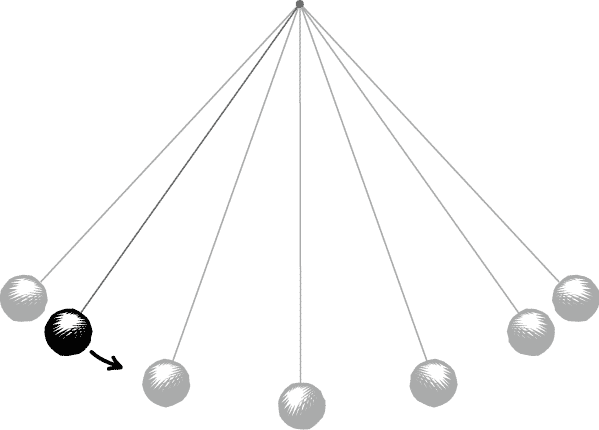
\includegraphics[width=0.6\linewidth]{Pictures/pendulum13}			
					\end{center}
				\end{column}	
				\begin{column}{.40\linewidth}
					\begin{center}
						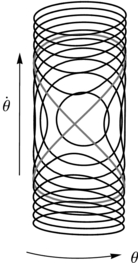
\includegraphics[width=0.45\linewidth]{Pictures/pendulum-phase-space}			
					\end{center}
				\end{column}	
			\end{columns}
			%
			\begin{defblock}[Symplectic Manifold]
				\vspace{-1em}
				\includestandalone[width=1\textwidth]{Pictures/Figure_sym}	
			\end{defblock}
			%
			\pause
			\begin{exblock}[$M = T^\ast Q$ is symplectic]
				with $\omega = d \theta $ given by
				$$ \left.\theta\right\vert_{(q,p)} (v) = p (\pi_\ast v) ~.$$
			\end{exblock}
			%
			\pause
			\vspace{1.2em}
			\centering
			\textit{ based on the notion of \\"states".}		
		\end{column}
		\onslide<1->{\vrule{}}
		\pause
		\begin{column}{.50\linewidth}
			\centering
			\textit{ "algebraic approach" to mechanics \dots}
			\vspace{.5em}	
			\begin{defblock}[Classical Observables]
				Unital, associative, commutative algebra $C^\infty(M)$.
			\end{defblock}
			%
			\vspace{.1em}
			\pause
			\begin{defblock}[Hamiltonian vector fields]
				$\vHam_f \in \mathfrak{X}(M)$ such that:
				$$\iota_{\vHam_f} \omega = -df \quad$$ %$\in B^1(M)$
				%
				\footnotetext{	$\vHam_f$ = \emph{Ham.v.f. pertaining to $f\in C^\infty(M)$}.}
			\end{defblock}
			\vspace{.1em}
			%
			\begin{defblock}[Poisson Algebra of Observables]
				$C^\infty(M)$ is a Poisson algebra with
				$$\{f,g\} = \iota_{\vHam_g} \iota_{\vHam_f} \omega = \omega(\vHam_f,\vHam_g) ~.$$
			\end{defblock}
			%
			\pause
			\vspace{.15em}
			\centering
			\textit{ based on the notion of \\"measurable quantities".}						
		\end{column}
	\end{columns}
\end{frame}
\note[itemize]{
		\footnotesize 
		\item We work in the framework of multisymplectic geometry which is one of the possible generalizations of the well-established field of symplectic geometry.
		\item To recall what symplectic geometry is let me assume a particular point of view: mechanics.
		\\
		Idea:"
		Symplectic geometry is a branch of differential geometry studying symplectic manifolds; it originated as a formalization of the mathematical apparatus of classical mechanics and geometric optics."{\href{https://ncatlab.org/nlab/show/symplectic+geometry}{nlab}}
		\\
		Namely, a sym. mfd. is the geometric structure encoding the phase space of conservative, autonomous, ordinary, classical, mechanical systems.
		\item 	{Geometrically: a Symplectic manifold $(M,\omega)$} $M$ a smooth manifold, $\omega\in \Omega^{2}(M)$ closed and non-degenerate, i.e. $d\omega=0$ and  $\omega^\flat:TM\to T^*M, v\mapsto \iota_v\omega$ is injective.
		\item
		Examples: orientable 2-manifolds with volume (e.g. $S^2$, $T^2$, $\mathbb R^2$), cotangent bunlde $T^*Q$ of any manifold $Q$ (with $\omega=d\theta$, $\theta_\eta(v)=\eta(T\pi_Q(v))$), coadjoint orbits. 
		\item $\theta$ = \emph{tautological 1-form}.
			$\theta$ evaluated at $p\in T^*Q$ in the fibre of $q\in Q$ and contracted with $v$ coincides with the form $p$ evaluated at $q$ and contracted with the push forward of $v$.
		\item We identify a special class of vector fields.
			Out of them one can define a Lie bracket.
		\item Poisson is a Lie algebra with the extra property of compatibility with the associative product (Leibniz rule)
		\item take away message: geometric (based on "states") vs algebraic (based on "measurable quantities").

}
%- . - . - . - . - . - . - . - . - . - . - . - . - . +

 




%-----------------------------------------------------------%
\subsection{Multisymplectic geometry}
%-----------------------------------------------------------%
 
%- . - . - . - . - . - . - . - . - . - . - . - . - . - . - . - . - . - . - . - . - . - . - . - .%
\begin{frame}{From symplectic to {multi}symplectic} 
	%
	\begin{center}
		$-$ \emph{multisymplectic means \textbf{going higher} in the degree of $\omega$} $-$
	\end{center}
	\pause
	\begin{defblock}[$n$-plectic manifold ~\emph{(Cantrijn, Ibort, De Le\'on)} \cite{Cantrun2017}]
		\includestandalone[width=0.95\textwidth]{Pictures/Figure_multisym}	
	\end{defblock}
	%
	\pause
		\begin{table}
			\begin{tabular}{c c c}
				symplectic forms \small($n=1$) & $\leftrightsquigarrow$ & volume forms \small($n= \text{dim}(M)-1$)
			\end{tabular}
		\end{table}

	\vfill
	\pause
	\begin{block}{Historical motivation}
		Mechanics: geometrical foundations of \textit{(first-order)} field theories.
	\end{block}
	%
	\begin{table}
		\ifHandout
		%
		\else
		\only<4>{
		\begin{tabular}{|p{0.2\textwidth}|p{0.3\textwidth}|p{0.35\textwidth}|} 
            \hline
            \parbox[][20pt][c]{0.2\textwidth}{mechanics} & \multicolumn{2}{c|}{geometry} \\
            \hline
            \parbox[][20pt][c]{0.2\textwidth}{phase space} & symplectic manifold &  \\[.25em]
            \parbox[][20pt][c]{0.2\textwidth}{classical \\ observables} & Poisson algebra &  \\[.25em]
            \parbox[][20pt][c]{0.2\textwidth}{symmetries} &  group actions admitting comoment map &  
            \\
            \hline
  \multicolumn{1}{c}{}
            &  \multicolumn{1}{@{}c@{}}{$\underbrace{\hspace*{.3\textwidth}}_{\text{point-like particles systems}}$} 
            &  \multicolumn{1}{@{}c@{}}{}              \\
		\end{tabular}
		}
		\fi
		\onslide<5->{
		\begin{tabular}{|p{0.2\textwidth}|p{0.3\textwidth}|p{0.35\textwidth}|} 
            \hline
            \parbox[][20pt][c]{0.2\textwidth}{mechanics} & \multicolumn{2}{c|}{geometry} \\
            \hline
            \parbox[][20pt][c]{0.2\textwidth}{phase space} & symplectic manifold & multisymplectic manifold \\[.25em]
            \parbox[][20pt][c]{0.2\textwidth}{classical \\ observables} & Poisson algebra & $L_\infty$-algebra \\[.25em]
            \parbox[][20pt][c]{0.2\textwidth}{symmetries} &  group actions admitting comoment map & group actions admitting (homotopy) comomentum map
            \\
            \hline
  			\multicolumn{1}{c}{}
            &  \multicolumn{1}{@{}c@{}}{$\underbrace{\hspace*{.3\textwidth}}_{\text{point-like particles systems}}$} 
            &
            \multicolumn{1}{@{}c@{}}{$\underbrace{\hspace*{.3\textwidth}}_{\text{field-theoretic systems}}$} 
               \\
		\end{tabular}
		}
	\end{table}	




\end{frame}
\note[itemize]{
	\item Historically, the interest in multisymplectic manifolds, has been motivated by the need for understanding the geometrical foundations of first-order classical field theories.
	The key point is that, just as one can associate a symplectic manifold to an ordinary classical mechanical system (e.g. a single
point-like particle constrained to some manifold), it is possible to associate a multisymplectic
manifold to any classical field system (e.g. a continuous medium like a filament or a fluid). See frame Extra-\ref{Frame:Ms-Field-Mechanics} 
	
	\item General ideas basic parallelisms with caveats
	\item caveat: points in multiphase spaces are not states
	\item the table hides the duality between geometric and algebraic approaches to the problem.
	\item	Mechanics: geometrical foundations of \textit{(first-order)} field theories.
		\begin{itemize}
		 \item[-] Kijowski, W. Tulczyjew \cite{Kijowski1979}; %(1979)
		 \item[-] Cariñena, Crampin, Ibort \cite{Carinena1991b};% (1991)
		 \item[-] Gotay, Isenberg, Marsden, Montgomery \cite{Gimmsy1};%(1998)
		 \\ $\cdots$
		\end{itemize}
	\item {Def. Multisymplectic manifold $(M,\omega)$}
	$M$ a smooth manifold, $\omega\in \Omega^{n+1}(M)$ closed and non-deg., i.e.: $d\omega=0$ and $\omega^\flat:TM\to \Lambda^nT^*M, v\mapsto \iota_v\omega$ is injective.
	\item Examples: orientable $n{+}1$-manifolds with volume (e.g. $S^{n+1}$, $T^{n+1}$, $\mathbb R^{n+1}$ ), multicotangent bunlde $\Lambda^nT^*Q$ of any manifold $Q$ (with $\omega=d\theta$. $\theta_\eta(v_1,...,v_n)=\eta(T\pi_Q(v_n),...,T\pi_Q(v_n))$),  semisimple Lie groups, hyperKähler manifolds,...
 	\item Without the non-deg. condition we call it \emph{premultisymplectic}. 

}
%- . - . - . - . - . - . - . - . - . - . - . - . - . - . - . - . - . - . - . - . - . - . - . - .%


%-----------------------------------------------------------%
\subsection{Higher Observables}
%-----------------------------------------------------------%

%- . - . - . - . - . - . - . - . - . - . - . - . - . - . - . - . - . - . - . - . - . - . - . - .%
\begin{frame}{Observables in $n$-plectic geometry}
	%
	\begin{defblock}[Hamiltonian $(n-1)$-forms]
		\begin{displaymath}
			\Omega^{n-1}_{ham}(M,\omega) 	:=
			\biggr\{ \sigma \in  \Omega^{n-1}(M) \; \biggr\vert \; 
				\exists \vHam_\sigma \in \mathfrak{X}(M) ~:~ 
				\tikz[baseline,remember picture]{\node[rounded corners,
                        fill=orange!5,draw=orange!30,anchor=base]            
            			(target) {$d \sigma = -\iota_{\vHam_\sigma} \omega$ };
            	}				
				~\biggr\} 
		\end{displaymath}
	\end{defblock}
%
%	\pause
%		\tikz[overlay,remember picture]
%		{
%			\node[rounded corners,
%                 fill=orange!5,draw=orange!30,anchor=base]
%            	 (base) at ($(current page.north east)-(2,1)$) [rotate=-0,text width=3.5cm,align=center] {\footnotesize{\textcolor{red}{Hamilton-DeDonder-Weyl \\equation}}};
%		}	
%	\begin{tikzpicture}[overlay,remember picture]
%    	\path[->] (base.south) edge[bend right,red](target.north);
%    \end{tikzpicture}
	%
	\vfill
	\begin{columns}[T]
		\pause
		\setlength{\belowdisplayskip}{5pt}
		\begin{column}{.50\linewidth}
			%
			\vspace{-1em}
			\begin{thmblock}[Observables $L_\infty$-algebra]
				$\Omega^{n-1}_{ham}(M,\omega)$ endowed with
				\vspace{-.5em}
				\begin{displaymath}
					\lbrace \sigma_1, \sigma_2 \rbrace =			
					~ - \iota_{\vHam_1}\iota_{\vHam_2} \omega 
				\end{displaymath}			
				can be "completed" to a \\ $L_\infty$-algebra.
			\end{thmblock}
			%	
		\end{column}	
		%
		\pause
		\begin{column}{.50\linewidth}
		%
			\begin{itemize}
				\item[\cmark] Skew-symmetric;
				\item[\xmark] multiplication of observables;
				\item[\xmark] Jacobi equation;
				%\\ \hspace*{4.25em} full-fledged Jacobi equation;
				\item[\smark] Jacobi equation \emph{up to homotopies}.
			\end{itemize}			
			%
				\[
					\small
					\{\alpha,\{\beta,\gamma\}\} + \text{\it cyc. perm.}
					= {\color{orange}\d \iota_{X_\alpha} \iota_{X_\beta} \iota_{X_\gamma}\omega}
				\]
		\end{column}	
	\end{columns}
	%
	\vfill
	\pause
	Interesting alternatives:
	\begin{itemize}
		\item  descend to $\Omega^{n-1}_{ham}(M) / {\color{orange}\d\hspace{1pt}\Omega^{n-2}(M)}$, hence getting a Lie algebra;
		\item Incorporate the {\color{orange}discrepancy} as part of the data of the space of observables 
				$L_\infty(M,\omega) = \Omega_{ham}^{n-1}(M)\oplus{\color{orange}\Omega^{\leq n-2}(M)}$.
			%a \textbf{homotopy Lie algebra} or \textbf{$L_\infty$-algebra}.
	\end{itemize}
	
	
\end{frame}
\note[itemize]{
	\item In the paper 
 \href{https://www.sciencedirect.com/science/article/pii/S0393044018301189}{Invitation to Multisymplectic Geometry} \cite{RYVKIN20199}\	, the equation highlighted in orange, which defines Hamiltonian forms, is referred to as the Hamilton--DeDonder--Weyl equation---a somewhat imaginative extension compared to its traditional formulation in \href{https://en.wikipedia.org/wiki/De_Donder\%E2\%80\%93Weyl_theory}{De Donder--Weyl theory}. 
	\item a **Hamiltonian $(k-1)$-form** $\alpha \in \Omega^{k-1}(M)$ is one that admits a vector field $X$ (a *Hamiltonian field*) satisfying $i_X\omega = d\alpha$. We call the pair $(X,\alpha)$ a *Hamiltonian pair*. 
	\item Just as in the symplectic case $(k=1)$ where $\alpha$ is a 0-form (function) and $X$ its Hamiltonian vector field, here $\alpha$ plays the role of the observable (often called an $(k-1)$-form observable). 
	\item The collection of all such Hamiltonian forms (for various degrees) can be organized into a graded object, and Rogers showed that it carries a canonical **$L_\infty$-algebra structure** .
    \item  **Example:** For a 3-plectic manifold (degree 3 form $\omega$), one has Hamiltonian 1-forms: each 1-form $\alpha$ for which there exists $X$ with $i_X\omega = d\alpha$. These Hamiltonian pairs $(X,\alpha)$ form the degree-0 part of the observables. In addition, ordinary functions (0-forms) can be viewed as Hamiltonian 0-forms (with $X$ such that $i_X\omega = d(0) = 0$), and perhaps higher-degree observables appear up to degree 1 in this case. The resulting $L_\infty$ has non-trivial brackets of arity up to 2 (making it a *Lie 2-algebra* of observables, a kind of higher Poisson algebra). The 2-bracket extends the Poisson bracket, and a 3-bracket arises measuring the failure of the Jacobi identity (something that vanishes in the symplectic case but not in general). For a 4-plectic form, one would get a Lie 3-algebra, etc.
}
%- . - . - . - . - . - . - . - . - . - . - . - . - . - . - . - . - . - . - . - . - . - . - . - .%



%- . - . - . - . - . - . - . - . - . - . - . - . - . - . - . - . - . - . - . - . - . - . - . - .%
\begin{frame}[fragile,t]{$L_\infty$-algebra of Observables (higher observables) }
	Let be $(M,\omega)$ a $n$-plectic manifold.
	\begin{defblock}[$L_\infty$-algebra of observables ~\emph{(Rogers)} ~\cite{Rogers2010}]
		
		\hspace{.25em} $L\infty(M,\omega)$ is given by:
		
		\begin{itemize}
			\item[•] a cochain-complex $(L,\{\cdot\}_1)$ 
		\end{itemize}
		\begin{center}
		\ifHandout
			\includestandalone{Pictures/Figure_Observables}	
		\else
			\includestandalone{Pictures/Frame_Observables}
		\fi				
		\end{center}
		\onslide<2->{
			\begin{itemize}
				\item[•] with $n$ (skew-symmetric) multibrackets $(2 \leq k \leq n+1)$
			\end{itemize}
			\begin{center}
				\includestandalone{Pictures/Equation_Multibracket}	
			\end{center}
		}
		%
	\end{defblock}
  \end{frame}
 \note[itemize]{
	\item if symplectic manifolds are the symmetric take on mechanics, Poisson algebras are the algebraic counterpart.
 	\item A Lie algebra is associated to an ordinary symplectic manifold (its Poisson algebra).
	%(Underlying this is a Lie algebra, whose Lie bracket is the Poisson bracket.)
	Similarly, one associates an Lie-$n$ algebra to any $n$-plectic manifold.
 	% https://ncatlab.org/nlab/show/n-plectic+geometry 	 
 	 %https://ncatlab.org/nlab/show/Poisson+bracket+Lie+n-algebra
	 \item Basically, the higher observables algebra is a chunk of the de Rham complex of $M$ with inverted grading( convention employed here) and an extra structure called "multibrackets".
 	\item ( In the 1-plectic case it reduces to the corresponding Poisson algebra of classical observables)
 	\item Rogers associated to any n-plectic mfd a $L\-\infty$ algebra, Zambon generalized it to the pre-n-plectic case.
 	\item Recognize in the definition of $\{\cdot,\ldots,\cdot\}_k$ the contraction with hamiltonian fields $v_\sigma$ w.r.t. $\sigma$.
  	\item Note $	\iota_{v_{\sigma_1}}\cdots\iota_{v_{\sigma_k}} = (-)^{(k-1)+(k-2)+\dots+1}\iota_{v_{\sigma_k}}\cdots\iota_{v_{\sigma_1}} = (-)^{\frac{k(k-1)}{2}}\iota_{v_{\sigma_k}}\cdots\iota_{v_{\sigma_1}}$ 
 	The definition usually find in literature of Rogers multibrackets involves the coefficient $ (-)^{\frac{k(k-1)}{2}} = -\varsigma(k-1) = (-)^{k+1} \varsigma(k)$.
  \item higher observables is Special instance of a more general object  called $L\-\infty$ Algebra...
 }
%- . - . - . - . - . - . - . - . - . - . - . - . - . - . - . - . - . - . - . - . - . - . - . - .%


 

%-----------------------------------------------------------%
%------------------------------------------------------------------------------------------------
\begin{frame}{Reminder: $L_\infty$ Algebras}

		\emph{
			$L_\infty$-algebra is the notion that one obtains from a Lie algebra when one requires the Jacobi identity to be satisfied only up to a higher coherent chain homotopy.
		}
		\\
		\vspace{.5em}
		\begin{defblock}[$L_\infty$-algebra ~\emph{(Lada, Markl, Stasheff)} ~\cite{Lada1993}\cite{Lada1995}]
			\includestandalone{Pictures/Figure_Linfinitydef}
		\end{defblock}	
		%
		%
	\pause
 

	\begin{itemize}
		\item<2-> You can construct a coalgebra out of $L$ \\
			{\small \color{UniGreen} (the reduced cofree coalgebra $S^{\geq 1}(L[1]),\Delta)$)}.
		\item<3-> You can assemble all $\mu_k$ to get a coderivation $Q_\mu$\\
				{\small \color{UniGreen} (the unique lift to a coderivation of the decalage of $ \mu=	\mu_1+\mu_2 + \dots$) }.
		\item<4-> Higher Jacobi is tantamount to having $Q_\mu ^2 = 0$.
	\end{itemize}
\end{frame}
\note[itemize]{
	\item $L_\infty$-algebra is the notion obtained from a Lie algebra requiring that the Jacobi identity is satisfied only up to a higher coherent chain homotopy.
	\item The Lie-n algebra mentioned before is a $L_\infty$ algebra with underlying graded vector space concentrated in degrees $0,1...n$.
	
	\item Definition. We say that a permutation $\sigma \in S_n$ is a $(j,n-j)$-unshuffle, $0\leq j \le1 n$  if $\sigma(1)< \dots < \sigma(j)$ and $\sigma(j+1)<\dots<\sigma(n)$.
	\\
	You can also say that $\sigma$ is a $(j,n-j)$-unshuffle if $\sigma(i)< \sigma(i+1)$ when $i\neq j$.

	\item 	Alternatively, the Jacobiators can be also denoted as $$\displaystyle J_m=\sum_{i+j=m+1} 	\mu_i \triangleleft \mu_j = 0$$
	employing the so-called \emph{ Richardson-Nijenhuis product}
		 $$\mu_i\circ \mu_j := (-)^{i(j+1)}\frac{1}{j!(i-1)!}\mu_i \triangleleft \mu_j\otimes \mathbb{1}_{i-1} \circ \mathcal{A}~,$$
		 where $\mathcal{A}$ denotes the (graded) total skew-symmetrizator.
		 
	\item see frame extra-\ref{Frame:unwapping-Jacobi} for a slightly demystification of the higher Jacobi equations.

	\item more precisely this statement is a proposition/definition

}
%------------------------------------------------------------------------------------------------


%%-----------------------------------------------------------%
%-----------------------------------------------------------%
\subsection{Goals}
%-----------------------------------------------------------%

%-----------------------------------------------------------%
\begin{frame}[fragile]{Scope / Goals}
	\begin{block}{Upshots:}
		\begin{itemize}
			\item[$\bullet$] Observables $L_\infty$-algebra construction is purely algebraic!
			\begin{itemize}
				\item[$\cdot$] \emph{(It relies only on the \underline{standard Cartan calculus identities} for differential forms and vector fields.)}
			\end{itemize}\pause
			\item[$\bullet$] Possible generalization to \underline{BV-modules over a Gerstenhaber algebra!}
			\begin{itemize}
				\item[$\cdot$] \emph{(A suitably general framework to formalize Cartan calculus.)}
			\end{itemize}
		\end{itemize}
	\end{block}
	\pause \vfill

	\begin{block}{Claim:}
		To any given BV-module over a Gerstenhaber algebra together with a chosen closed element (a "cocycle") in the module, we can define:
		\begin{itemize}
			\item[$\cdot$] Hamiltonian pairs,
			\item[$\cdot$] together with an associated $L_\infty$-algebra structure.
		\end{itemize}
	\end{block}
	\pause \vfill

	\begin{block}{Applications:}
		\begin{itemize}
			\item[$\bullet$] A more conceptual picture for the algebraic reduction of the observables $L_\infty$-algebra in presence of constraints / symmetries.
		\end{itemize}
	\end{block}
	\vfill

\end{frame}
\note[itemize]{
	\item   Cartan's identities ensure that the operations $d, i_X, L_X$ behave in a coordinated way (the essence of *Gerstenhaber algebra and BV-module* structure, as we formalize below). 
	\item Rogers’ $L_\infty$ brackets are built using these ingredients: e.g., the binary bracket of two Hamiltonian forms $(X,\alpha)$ and $(Y,\beta)$ can be defined as $( [X,Y],; L_X\beta)$ (or plus cyclic terms), and higher brackets involve expressions with $i_{X_i} i_{X_j}\omega$ contracted with another argument, etc., ensuring the homotopy Jacobi identities hold .
	\item The key point is that all such formulas **only use the algebraic operations $d,i,L,[\cdot,\cdot]$ and the form $\omega$**. This algebraic nature allows generalization to any context where similar operators exist.
	\item *Limitations of Classical Reduction:** Before moving to the algebraic setup, note that reducing multisymplectic systems geometrically (analogue of Marsden-Weinstein reduction) can be challenging. Classical symplectic reduction requires a Lie group action that is free and proper and a regular value of the moment map; these conditions often fail (especially in field theory or higher form cases). Recent work has approached reduction **algebraically** by focusing on the algebra of observables (functions/forms) with constraints, rather than the quotient of manifolds. This algebraic approach, implemented for multisymplectic manifolds in Blacker-Miti-Ryvkin 2024, allows handling singular cases (non-free actions, etc.) by *encoding constraints and symmetries at the algebraic level.
Our work builds on this idea using *constraint triples*.
\item Given any Gerstenhaber algebra $G$ together with a BV-module $M$ and a chosen closed element (a  "cocycle ") $c$ in $M$, we will show how to construct an associated $L_\infty$-algebra of observables without reference to any underlying manifold .
\item Moreover, we will address how to perform reduction of these observables $L_\infty$-algebras in the presence of constraints or symmetries. For this, we employ the notion of constraint triples as an algebraic framework for coisotropic reduction. Adapting this to our BV-module setting, we obtain a general procedure to reduce an $L_\infty$ of observables, even in singular scenarios where classical quotient constructions fail  
}
%-----------------------------------------------------------%	

 


%-----------------------------------------------------------%
\ifstandalone
% https://en.wikibooks.org/wiki/LaTeX/Bibliographies_with_biblatex_and_biber
\begin{frame}[t,allowframebreaks]{Bibliography}
	%\nocite{*}
	\printbibliography
\end{frame}
\fi
%-----------------------------------------------------------%


%-----------------------------------------------------------+
\end{document}
%-----------------------------------------------------------+



%+----------------------------------------------------------+



%+----------------------------------------------------------+
\section{BV-Modules: Algebraic Cartan Calculus}
%+----------------------------------------------------------+
	\checkpoint	
	%- HandOut Flag ----------------------
\makeatletter
\@ifundefined{ifHandout}{%
  \expandafter\newif\csname ifHandout\endcsname
}{}
\makeatother

%- D0cum3nt ----------------------------------------------------------------------------------------------
%\documentclass[beamer,10pt]{standalone}   
\documentclass[beamer,10pt,handout]{standalone}  \Handouttrue  

\ifHandout
	\setbeameroption{show notes} %print notes   
\fi

	
%- Packages ----------------------------------------------------------------------------------------------
\usepackage{custom-style}
\usepackage{math}



%--Beamer Style-----------------------------------------------------------------------------------------------
\usetheme{toninus}
\usepackage{animate}
\usetikzlibrary{positioning, arrows}
\usetikzlibrary{shapes}


%- Bibliography (Biber) ----------------------------------------------------------------------------------
\usepackage[backend=biber,style=alphabetic,maxnames=2]{biblatex}
\bibliography{bibfile.bib}

%===========================================================%
\begin{document}
%===========================================================%
\checkpoint


%-----------------------------------------------------------+
\begin{frame}{Lie-Rinehart Algebras}

  \begin{defblock}[Lie-Rinehart Algebra]
    A pair $(A,E)$ where
    \begin{itemize}
      \item $A$ is a commutative, associative algebra,
      \item $E$ is an $A$-module and a Lie algebra,
      \item there is an anchor map $\rho: E \to \mathrm{Der}(A)$ satisfying the Leibniz rule:
        \[
          [X, aY] = a[X,Y] + (\rho(X)a)Y, \quad \forall X,Y \in E, a \in A.
        \]
    \end{itemize}
  \end{defblock}  


\begin{itemize}
  \item Encodes derivations + Lie algebra structure.
\end{itemize}

  \begin{exblock}
    If $A=C^\infty(M)$, then $E=\Gamma(TM)$ with $\rho=\mathrm{id}$ is a Lie-Rinehart algebra.

    Lie-Rinehart algebras are algebraic analogues of Lie algebroids (and every Lie algebroid gives a Lie-Rinehart algebra)
  \end{exblock}

\end{frame}
\note[itemize]{
  \item To generalize the above geometric structures, we introduce the algebraic counterparts of  "multivector fields " and  "differential forms with Cartan calculus. " 
  \item  A  Lie-Rinehart algebra  $(A,E)$ consists of a commutative associative algebra $A$ (think of $A=C^\infty(M)$) and an $A$-module $E$ (think of $E=\mathfrak X(M)$, the vector fields) which is also a Lie algebra, together with an *anchor* map $\rho: E \to \mathop{\mathrm{Der}}(A)$ (derivations of $A$) satisfying a Leibniz rule: $[X, aY] = a[X,Y] + (\rho(X)a),Y$. This abstractly encodes the notion of derivations of $A$ with an $A$-linear Lie bracket. 
  \item Example: If $A=C^\infty(M)$, then $E=\Gamma(TM)$ (the module of vector fields) with the identity anchor $\rho(X)=X$ is a Lie-Rinehart algebra. 
  \item   In fact, Lie-Rinehart algebras are algebraic analogues of Lie algebroids (and every Lie algebroid gives a Lie-Rinehart algebra).}
%-----------------------------------------------------------+


%-----------------------------------------------------------+
\begin{frame}{Gerstenhaber Algebras}
  \emph{A graded algebra that captures the structure of exterior algebra of multivector fields.}
  %
  \begin{defblock}[Gerstenhaber Algebra]
    A triple $(\mathcal{G}, \wedge, [\cdot,\cdot])$ where
    \begin{itemize}
      \item $\mathcal{G} = \bigoplus_{i\in\mathbb{Z}} \mathcal{G}^i$ is a $\mathbb{Z}$-graded vector space,
      \item $\wedge: \mathcal{G}^p \times \mathcal{G}^q \to \mathcal{G}^{p+q}$ is a graded-commutative, associative product (degree $0$ operation),
      \item $[\cdot,\cdot]: \mathcal{G}^p \times \mathcal{G}^q \to \mathcal{G}^{p+q-1}$ is a bracket of degree $-1$, making $\mathcal{G}$ into a graded Lie algebra,
      \item Compatibility (Leibniz rule): The bracket is a derivation of the product:
        \[
          [x, y\wedge z] = [x,y]\wedge z + (-1)^{(\deg x -1)\deg y} y\wedge [x,z]
        \]
        for homogeneous $x,y,z$.
    \end{itemize}

    \begin{exblock}%{Example}
      If $(A,E)$ is a Lie-Rinehart algebra, the exterior algebra of $E$ (with a degree shift) carries a natural Gerstenhaber structure.
    \end{exblock}

    \begin{exblock}%{Example}
      Take $\mathcal{G} = \Lambda^\bullet E$ (the exterior wedge algebra of $E$ treated as a graded space of multivectors). The wedge product is the usual wedge of multivectors, and the bracket is the Schouten-Nijenhuis bracket extending the Lie bracket on $E$ to all multivectors. This $(\Lambda E,\wedge,[\cdot,\cdot]_{SN})$ is a Gerstenhaber algebra, prototypical in geometry (for $E=\mathfrak X(M)$ one recovers the standard Gerstenhaber algebra of multivector fields on $M$).
    \end{exblock}
 
\end{frame}
\note[itemize]{
  \item  A Gerstenhaber algebra is a graded algebra that captures the structure of exterior algebra of multivector fields. 
  \item Compatibility (Leibniz rule): The bracket is a derivation of the product: $[x, y\wedge z] = [x,y]\wedge z + (-1)^{(\deg x -1)\deg y} y\wedge [x,z]$ for homogeneous $x,y,z$. This is the defining Gerstenhaber identity, generalizing the fact that the Lie bracket of vector fields satisfies a Leibniz rule with respect to wedge of forms or functions.
}
%-----------------------------------------------------------+



%-----------------------------------------------------------+
\begin{frame}{Gerstenhaber Modules}
  %
  \begin{defblock}[Gerstenhaber Module]
    A Gerstenhaber module over a Gerstenhaber algebra $(\mathcal{G}, \wedge, [\cdot,\cdot])$ is a graded module $\mathcal{M} = \bigoplus_{i\in\mathbb{Z}} \mathcal{M}^i$ together with an action
    \[
      \iota: \mathcal{G}^p \times \mathcal{M}^q \to \mathcal{M}^{q - p}
    \]
    satisfying:
    \begin{itemize}
      \item $\iota$ is $A$-linear in the second argument,
      \item **Compatibility:** For homogeneous $x,y\in \mathcal{G}$ and $m\in \mathcal{M}$,
        \[
          \iota_{[x,y]} m = \iota_x (\iota_y m) - (-1)^{(\deg x -1)(\deg y -1)} \iota_y (\iota_x m).
        \]
    \end{itemize}


\begin{itemize}
  \item $G$-module $M$ with contraction $\iota_X$ of degree $-\deg X$.
  \item Induced Lie derivative $L_X = [d,\iota_X]$ when $d$ is defined.
\end{itemize}
\end{frame}
\note[itemize]{
  \item Gerstenhaber Module extends the idea of a multivector acting on forms by contraction. 
  \item Concretely, for each element $X\in G^p$, we have a degree $-p$ operator $i_X: M^\ast \to M^{\ast-p}$ (interpreted as interior product by $X$) satisfying a compatible set of identities (graded derivations, etc.). 
  \item We also typically get an induced Lie derivative action $L_X$ of degree 0 defined by $L_X := [D,;i_X]$ once a differential $D$ is present (see below). We won’t detail the full set of axioms here, but essentially a Gerstenhaber module gives an algebraic version of the pair of operations $(i_X, L_X)$ acting on a  "forms " module, with $i$ being antiderivations and $L$ Lie derivations.
  \item (The literature sometimes refers to this structure as a  "TTN (Tsygan-Tamarkin-Nest) calculus " .)}
%-----------------------------------------------------------+


%-----------------------------------------------------------+
\begin{frame}{BV-Modules}
  %
  \begin{defblock}[Batalin-Vilkovisky Module]
    A Batalin-Vilkovisky module (BV-module) over a Gerstenhaber algebra $(\mathcal{G}, \wedge, [\cdot,\cdot])$ is a Gerstenhaber module $(\mathcal{M}, \iota)$ together with a differential $d: \mathcal{M}^i \to \mathcal{M}^{i+1}$ (i.e. $d^2=0$) satisfying the Cartan identity:
    \[
      L_x := [d, \iota_x] = d \circ \iota_x + (-1)^{\deg x -1} \iota_x \circ d
    \]
    for all homogeneous $x\in \mathcal{G}$, where $L_x$ is the Lie derivative induced by the Gerstenhaber module structure.
  \end{defblock}

\end{frame}
\note[itemize]{
  \item Batalin-Vilkovisky Modules (BV-Modules): A BV-module is a Gerstenhaber module that is also equipped with a differential of degree $+1$ (like an exterior derivative) satisfying Cartan’s formula. 
  \item Formally, let $G$ be a Gerstenhaber algebra and $(M,d)$ a cochain complex (so $d: M^i \to M^{i+1}$ with $d^2=0$). We say $M$ is a BV-module over $G$ if $M$ is a Gerstenhaber $G$-module and, for all $X\in G$, we have the Cartan identity $L_X = [d,; i_X]$ (and automatically $[L_X, i_Y] = i_{[X,Y]}$, etc.)  . 
  \item In other words, $M$ carries an action of $G$ by contraction $i_X$ and Lie derivative $L_X$ such that together with the differential $d$ they satisfy the standard graded commutation relations of Cartan calculus. \item We often call $d$ the BV differential.}
%-----------------------------------------------------------+


%-----------------------------------------------------------+
\begin{frame}{Abstract Cartan Calculus}
\begin{itemize}
  \item A Gerstenhaber module $M$ with differential $d$.
  \item Cartan identity: $L_X = [d,\iota_X]$.
  \item Encodes full algebraic Cartan calculus.
\end{itemize}


  \begin{itemize}
  \item $(G,M,d)$ with $G$ Gerstenhaber, $M$ BV-module, $d^2=0$.
  \item Examples: $(\mathfrak{X}^\bullet(M),\Omega^\bullet(M), d)$.
  \item Extends to noncommutative and algebraic settings.
\end{itemize}
\end{frame}
\note{Example (Classical Cartan Calculus): Take $G = \Lambda^\bullet \mathfrak X(M)$ (Gerstenhaber algebra of multivector fields on a manifold) and $M=\Omega^\bullet(M)$ (the de Rham complex of differential forms). This is a canonical example of a BV-module  : the differential $d$ is the exterior derivative, the contraction $i_X$ is the usual insertion of a multivector $X$ into a form, and the Lie derivative $L_X$ is the usual one acting on forms. These satisfy $L_X = d \circ i_X + i_X \circ d$ (Cartan formula) and all other Cartan identities. In fact, this example exactly recovers the classical Cartan calculus on $M$ as a BV-module structure on $\Omega^\bullet(M)$, with $G$ playing the role of  "polyvector fields " . This justifies the abstractions: any Gerstenhaber algebra + BV-module pair can be seen as a generalized  "space of multivectors and forms " with a full Cartan calculus available . We emphasize that such structures exist in much more general settings, including noncommutative geometry (where $A$ is a noncommutative algebra and one considers analogues of forms and multivectors  ), but for our purposes we stick to the algebraic axioms.}
%-----------------------------------------------------------+


%-----------------------------------------------------------%
\ifstandalone
% https://en.wikibooks.org/wiki/LaTeX/Bibliographies_with_biblatex_and_biber
\begin{frame}[t,allowframebreaks]{Bibliography}
	%\nocite{*}
	\printbibliography
\end{frame}
\fi
%-----------------------------------------------------------%


%-----------------------------------------------------------+
\end{document}
%-----------------------------------------------------------+





%-----------------------------------------------------------%

%+----------------------------------------------------------+
\section{$L_\infty$ Algebra Associated with a BV-Module}
%+----------------------------------------------------------+
	\checkpoint	
	%%- HandOut Flag ----------------------
\makeatletter
\@ifundefined{ifHandout}{%
  \expandafter\newif\csname ifHandout\endcsname
}{}
\makeatother

%- D0cum3nt ----------------------------------------------------------------------------------------------
%\documentclass[beamer,10pt]{standalone}   
\documentclass[beamer,10pt,handout]{standalone}  \Handouttrue  

\ifHandout
	\setbeameroption{show notes} %print notes   
\fi

	
%- Packages ----------------------------------------------------------------------------------------------
\usepackage{custom-style}
\usepackage{math}



%--Beamer Style-----------------------------------------------------------------------------------------------
\usetheme{toninus}
\usepackage{animate}
\usetikzlibrary{positioning, arrows}
\usetikzlibrary{shapes}


%- Bibliography (Biber) ----------------------------------------------------------------------------------
\usepackage[backend=biber,style=alphabetic,maxnames=2]{biblatex}
\bibliography{bibfile.bib}

%===========================================================%
\begin{document}
%===========================================================%
\checkpoint

%-----------------------------------------------------------%
\begin{frame}[fragile]{Abstract Hamiltonian Pairs}
  \begin{quote}
    \emph{Rogers construction naturally generalizes to a purely algebraic setting.}
  \end{quote}
  \vfill\pause

  Data:
  \begin{itemize}
    \item $G = (G,\wedge,\lbrace \cdot, \cdot \rbrace)$ a Gerstenhaber algebra;
    \item $V = (V,\d,\iota,\Lie)$ a BV-module over $G$;
    \item $\omega \in V^{k{+}1}$ a fixed cocycle, i.e. $\d \omega = 0$, for $k\geq 1$.
  \end{itemize}
  \vfill\pause

  \begin{defblock}[Hamiltonian Pairs]
    Elements of the graded vector space:
	  $$
		\Ham^0(V, \omega) := \left\{ (\alpha, X) \in V^{k-1} \oplus G^1 \mid \iota_X \omega = -\d\alpha \right\},
    $$
  \end{defblock}
  \vfill\pause

  \begin{remblock}[$\Ham^0(V, \omega)$ can also be viewed as the fibered product \( V^{k-1} \times_{V^k} G^1 \)]
     over the following pullback in the category of vector spaces:
	\begin{displaymath}
		\begin{tikzcd}
			\Ham^0(V, \omega) \arrow[r] \arrow[d] \ar[dr,"\lrcorner",very near start,phantom]& G^1 \ar[d,"\iota_{\blank}\omega"] \\
			V^{k-1} \arrow[r, "-\d"] & V^{k}
		\end{tikzcd}
	\end{displaymath}
  \end{remblock}
\end{frame}
\note[itemize]{
  \item The construction of the Roger's $L_\infty$-algebra  can be carried out for any BV-module equipped with a fixed $k+1$-cocycle $\omega$, i.e., for which $\d \omega = 0 $ with respect to the differential $\d$, since being a BV-module provides the structure of a complete Cartan calculus, which is all we need. 
}
%-----------------------------------------------------------%


%-----------------------------------------------------------%
\begin{frame}{Abstract {$L_\infty$}-algebra of Observables}


\begin{defblock}[{$L_\infty$}-algebra of Observables]
  The graded vector space $\Ham(V, \omega)$  given by
  $$
  \Ham(V, \omega)^i := \begin{cases}
    V^{k-1 + i} & i \leq -1, \\
    \Ham^0(V, \omega) & i = 0,\\
    0 & i \geq 1~;
  \end{cases} 
  $$
  with degree $(2-j)$ multibrackets $l_j\colon \Ham^{\otimes j}(V, \omega) \to \Ham(V, \omega)[2-j]$, given by:

	\begin{itemize}
		\item $
			      l_1(\alpha) = \begin{cases}
				      \d\alpha      & \text{if } i < -1, \\
				      (\d\alpha, 0) & \text{if } i = -1, \\
				      0             & \text{if } i = 0;
			      \end{cases} $\\
		\item $
        l_2\big( (\alpha_1, X_1), (\alpha_2, X_2) \big) = \big( \iota_{X_1} \iota_{X_2} \omega, \{X_1, X_2\} \big);
		      $\\
		\item $
          l_{j\geq 3}\big( (\alpha_1, X_1), \dots, (\alpha_j, X_j) \big) = -\iota_{X_1} \dots \iota_{X_j} \omega;
		      $\\
		\item All multibrackets of arity greater than or equal to $2$ vanish when evaluated on at least one degree nonzero element.
	\end{itemize}
\end{defblock}
%


\end{frame}
\note[itemize]{
    \item 	The verification that the above definition yields an honest $L_\infty$-algebra can be directly adapted from~\cite[Thm. 5.2]{rogers2012linfty} noticing that their proof is purely algebraic in nature and relies only on the Cartan calculus axioms.
}
%-----------------------------------------------------------%

%-----------------------------------------------------------%
\begin{frame}[fragile]{Abstract {$L_\infty$}-algebra of Observables (examples)}

  \begin{exblock}[Observables $L_\infty$-algebra associated with a Lie--Rinehart algebra]
    Let $(A, \mathfrak{L})$ be a Lie--Rinehart algebra, $\omega \in \CE(\mathfrak{L})^{k+1}$ a cocycle.
    \\
    We get an $L_\infty$-structure on the complex
	\begin{displaymath}
		\begin{tikzcd}[]
			A \arrow[r] &
			\mathfrak{L}^* \arrow[r] &
			\cdots \arrow[r] &
			(\Lambda^{k-2} \mathfrak{L})^* \arrow[r] &
			(\Lambda^{k-1} \mathfrak{L})^* \times_{(\Lambda^k \mathfrak{L})^*} \mathfrak{L}
		\end{tikzcd}~.
	\end{displaymath}
\end{exblock}
  \vfill\pause

\begin{exblock} 
	When 
   $$ A=C^\infty(M)~, \qquad  \mathfrak{L}=\mathfrak{X}(M)$$
   we retrieve the Roger's construction (given in the context of closed differential forms).
\end{exblock}

\end{frame}
\note[itemize]{
    \item b
}
%-----------------------------------------------------------%




%-----------------------------------------------------------%
\ifstandalone
% https://en.wikibooks.org/wiki/LaTeX/Bibliographies_with_biblatex_and_biber
\begin{frame}[t,allowframebreaks]{Bibliography}
	%\nocite{*}
	\printbibliography
\end{frame}
\fi
%-----------------------------------------------------------%



%-----------------------------------------------------------+
\end{document}
%-----------------------------------------------------------+

%===========================================================%





We now turn to the second main part: **reduction** of the $L_\infty$-algebra of observables in the presence of constraints or symmetries. In symplectic geometry, reduction is accomplished by the Marsden-Weinstein quotient: one restricts to the zero level set of a momentum map and then quotients by the symmetry group. Algebraically, this corresponds to first imposing ideal relations (for the constraints) and then modding out by gauge symmetries. The **constraint triple** formalism packages these two steps (subobject and quotient) in a single algebraic structure .

- **Constraint Triples:** A **constraint triple** (or **coisotropic triple**) in general consists of:
    1. An algebra (or other structure) $A$ representing the full system’s observables.
    2. A subalgebra $C \subset A$ representing the *constraints* (for example, functions vanishing on a certain submanifold, or first-class constraint algebra in Dirac’s theory).
    3. A quotient (factor) algebra $\overline{A} = A/ I$ for some ideal $I$ related to $C$, representing the *reduced* algebra of observables after constraints are imposed and quotiented.
    
    These are equipped with structure maps (inclusions and projections) satisfying compatibility conditions (e.g. $I$ is the ideal of relations defining $C$) . Intuitively, one has $C$ as the "constraint algebra" (functions that vanish on the constraint surface) and $\overline{A}$ as the algebra of functions on the quotient of that constraint surface by symmetries. Dippel, Esposito & Waldmann formalized this in the context of Poisson algebras and deformation quantization , showing that many reduction procedures can be understood as functors on such triples.
    
    We adopt this idea in our setting: we will consider **constraint Gerstenhaber algebras** and **constraint BV-modules**, which are triples $(G, G_C, \overline{G})$ and $(M, M_C, \overline{M})$ capturing the full, constraint, and reduced parts of our algebraic Cartan calculus . All the structure (brackets, differentials, etc.) is assumed to exist on each part and to be compatible. For instance, a *constraint Gerstenhaber algebra* means $G$ is a Gerstenhaber algebra, $G_C \subset G$ a subalgebra (constraints), and $\overline{G} = G/G_C$ (some quotient) such that the wedge and bracket operations map triples to triples (roughly $[![G, G]!]$ sends $G_C$ to $G_C$ and induces well-defined operations on the quotient) . Similarly, a *constraint BV-module* $(M, M_C, \overline{M})$ has $M_C$ a submodule (the  "constraints on forms ") and $\overline{M}=M/M_C$ the quotient module, with differential $d$ and contractions $i_X$ etc. respecting the triples (so that, e.g., $d(M_C)\subseteq M_C$ and induces a differential on $\overline{M}$) . This is a bit of structure to keep track of, but conceptually it means we have *Cartan calculus not just on one algebra, but simultaneously on a sub- and a quotient algebra*.
    
    - **Origin in Geometry:** If one has a manifold $M$ with a coisotropic submanifold $C\subset M$ (the constraint surface) and a group $G$ acting with gauge orbits, one can form a *constraint manifold* in the sense of Dippel-Kern 2025 . The algebra of smooth functions on a constraint manifold is exactly a constraint triple $(A, C, \overline{A})$ in which $C$ are the functions vanishing on the constraint surface and $\overline{A}$ functions on the quotient (when nice). Likewise, vector fields tangent to $C$ etc. form a constraint Lie-Rinehart algebra, and so on. Indeed, it has been shown that a **constraint Lie-Rinehart algebra** naturally induces a constraint Gerstenhaber algebra and constraint BV-module structures . So this framework is not lacking examples - it generalizes classical constrained Hamiltonian systems.
- **Constraint $L_\infty$ of Observables:** Once we have constraint versions of $G$ and $M$ **and** a *constraint cocycle* $c = (c, c_C, \overline{c})$ (meaning $c$ lies in $M$, $c_C$ in $M_C$ and $\overline{c}$ is its class in $\overline{M}$, with each closed under their respective differentials), we can perform the same construction as before *in the category of constraint complexes*. That is, we define the **constraint Hamiltonian pairs** as triples $((X, X_C, \overline{X}), (m, m_C, \overline{m}))$ such that $i_X(c) = d m$, $i_{X_C}(c_C) = d m_C$ and these are compatible/projection of the first (so $\overline{X}$ and $\overline{m}$ are the images of $X,m$, etc.) . All such triples form a constraint graded space of observables. **Theorem C** asserts that this constraint observables space carries a **constraint $L_\infty$-algebra** structure . By  "constraint $L_\infty$-algebra, " we mean an $L_\infty$ whose underlying structure is also a triple $(L, L_C, \overline{L})$: there are brackets $\ell_r$ on each of $L, L_C, \overline{L}$, and the inclusion/projection maps intertwine these (so that $L_C$ is an $L_\infty$-subalgebra and $\overline{L}$ the quotient $L_\infty$) . The brackets are defined using the same formulas as in the unconstrained case, applied levelwise to $(G, M, c)$, $(G_C, M_C, c_C)$ and inducing $(\overline{G}, \overline{M}, \overline{c})$ . The $L_\infty$ identities hold simultaneously on each level by the same reasoning as before, thanks to the compatibility of the constraint data.
- **Reduction Functor:** Once we have a constraint $L_\infty$-algebra of observables, *reducing it* means passing to the **quotient part** of the constraint triple. In categorical terms, there is a forgetful functor sending a constraint object $(X, X_C, \overline{X})$ to the quotient $\overline{X}$. When we apply this to the constraint $L_\infty$ of observables, we obtain an $L_\infty$-algebra on $\overline{L}$, which we interpret as the **reduced $L_\infty$-algebra of observables** of the constrained system. Intuitively, this $\overline{L}$ encodes observables that are invariant under the symmetry and defined on the constraint surface (since we mod out those that vanish or differ by constraint terms) . By construction, all the $L_\infty$ brackets descend to $\overline{L}$, so the homotopy Lie structure is well-defined on the quotient. This algebra $\overline{L}$ is the algebraic analog of the Poisson algebra of the reduced phase space in classical reduction, but here it can handle the homotopy brackets arising from a multisymplectic form and even if no nice manifold quotient exists (e.g. in singular cases).
- **Recovery of Known Results:** Our general reduction scheme, when applied to the **geometric case** of a multisymplectic manifold with a group action, reproduces the results of our earlier work (Blacker-Miti-Ryvkin, SIGMA 2024) . In that work, we constructed a reduced $L_\infty$ of observables by more ad-hoc means; now we see it fits into the constraint triple framework. Specifically, given a Lie group $G$ acting on an $n$-plectic manifold $(M,\omega)$ with a covariant momentum map $\mu$ , one can form the constraint triple:
    - $A = $ observables $L_\infty$ on $(M,\omega)$,
    - $A_C = $ those observables that vanish on the constraint (e.g. forms pulled back by $\mu$ setting to zero, etc.),
    - $\overline{A} = $ observables on the reduced space (when $0$ level set mod $G$ is nice, these correspond to forms on the quotient).
    
    Our formalism shows that $\overline{A}$ inherits an $L_\infty$-algebra structure automatically . No assumptions of regularity or freeness are needed in the algebraic approach - even if the quotient is singular, $\overline{A}$ is well-defined as a homotopy algebra. This extends the multisymplectic reduction of Blacker 2021 (which assumed regularity) to a far more general context . Moreover, within our algebraic setting we identify an object called the **residue defect**, which measures the slight difference between naive and actual reduction in the homotopy context. In the earlier work, this residue term appeared somewhat mysteriously to satisfy the homotopy Jacobi identities; here we can interpret it cleanly as arising from the constraint differential and the failure of a certain exactness on the constraint submodule. Our framework **clarifies the role of the  "residue defect "**: it is an intrinsic part of the constraint $L_\infty$ structure that vanishes under appropriate conditions (like when the momentum map level is regular) .
    
- **Summary of Main Results:** We can summarize the main technical results (theorems) as follows:
    - **Theorem A:** *Given any Gerstenhaber algebra $G$ with a BV-module $M$ and a closed element $c\in M$, the graded space of Hamiltonian pairs $\mathcal{O}(G,M;c)$ admits an $L_\infty$-algebra structure (observables algebra), defined by the multilinear maps derived from Cartan calculus.* 
    - **Theorem B:** *If $(A,E)$ is a **constraint** Lie-Rinehart algebra (constraint version of derivations over a constraint algebra $A$), then one naturally obtains a constraint Gerstenhaber algebra and a constraint BV-module $(G, M)$ out of it. (In short, classical constraint manifolds yield constraint Cartan calculus algebraically.)
    - **Theorem C:** *Given a constraint Gerstenhaber algebra and BV-module with a constraint cocycle $c$, one can construct a **constraint** $L_\infty$-algebra of observables. Moreover, its **reduced part** $\overline{\mathcal{O}}$ (the quotient level) is an $L_\infty$-algebra that describes the observables of the reduced system.* 
    
    As an application, Theorem C applied to multisymplectic manifolds with symmetries recovers the reduced $L_\infty$ in  and explains the extra terms (residue defect) in a categorical way .
    

## **Conclusion and Outlook**

We have developed a **purely algebraic toolkit** for constructing and reducing $L_\infty$-algebras of observables, extending concepts from symplectic geometry to multisymplectic and even noncommutative settings . This framework shows the power of combining homotopy algebra (for observables) with constraint category theory (for reduction). It provides a unified perspective where classical geometric reduction is just one instance of an algebraic functor acting on $L_\infty$-algebras .

Some directions for further research include:

- **Homotopy Momentum Maps:** Relating our constraint $L_\infty$-reduction to the notion of *homotopy momentum maps* (which appear in alternative higher reduction approaches, e.g. the work of Callies-Frégier-Rogers-Zambon on $L_\infty$-moment maps . It would be interesting to connect the **Leibniz-algebra-valued momentum maps** used here  with homotopy moment maps in an $L_\infty$-context.
- **Operadic Formulation:** The constraint triple constructions hint at an operadic or higher-categorical organization. One could aim to describe the entire process (Cartan calculus + constraints + $L_\infty$) in terms of operads or properads encoding these algebraic relations . This might streamline proofs and allow further generalizations (e.g. to quantum or $A_\infty$ settings).
- **Applications to Field Theory:** Ultimately, multisymplectic forms arise in classical field theory (e.g. the 2-form in mechanics vs. a 3-form in 2-dimensional field theory). Our algebraic observables $L_\infty$ could serve as a foundation for understanding *higher Poisson brackets* on the phase space of fields and their reduction under symmetries. Recent works on polysymplectic and polycontact reduction provide complementary geometric approaches; linking those with our algebraic method is a promising avenue.

**References:** *(Selected key references in context)* Rogers (2012) for the original multisymplectic $L_\infty$-algebra construction; Dippel-Esposito-Waldmann (2019) for constraint (coisotropic) triples in Poisson algebra setting; Blacker-Miti-Ryvkin (2024) for algebraic multisymplectic reduction; and our work Miti-Ryvkin (2025) (Differential Geom. Appl.) which this talk is based on, for full details and proofs. The methods presented exemplify how **pure algebraic techniques can not only recover but also enlighten classical geometric results** in higher symplectic geometry, broadening the scope to singular and noncommutative realms.
%-----------------------------------------------------------%

%+----------------------------------------------------------+
\section{An Application: Multisymplectic Reduction}
%+----------------------------------------------------------+
	\checkpoint	
	%%- HandOut Flag ----------------------
\makeatletter
\@ifundefined{ifHandout}{%
  \expandafter\newif\csname ifHandout\endcsname
}{}
\makeatother

%- D0cum3nt ----------------------------------------------------------------------------------------------
\documentclass[beamer,10pt]{standalone}   
%\documentclass[beamer,10pt,handout]{standalone}  \Handouttrue  

\ifHandout
	\setbeameroption{show notes} %print notes   
\fi

	
%- Packages ----------------------------------------------------------------------------------------------
\usepackage{custom-style}
\usepackage{math}



%--Beamer Style-----------------------------------------------------------------------------------------------
\usetheme{toninus}
\usepackage{animate}
\usetikzlibrary{positioning, arrows}
\usetikzlibrary{shapes}


%- Bibliography (Biber) ----------------------------------------------------------------------------------
\usepackage[backend=biber,style=alphabetic,maxnames=2]{biblatex}
\bibliography{bibfile.bib}

%===========================================================%
\begin{document}
%===========================================================% 
\checkpoint

%- . - . - . - . - . - . - . - . - . - . - . - . - . - . - . - . - . - . - . - . - . - . - . - .%	
\subsection{Regular reduction} 
%- . - . - . - . - . - . - . - . - . - . - . - . - . - . - . - . - . - . - . - . - . - . - . - .%	
\begin{frame}{Regular reduction in symplectic geometry}

	\textbf{\color{UniGreen}Symplectic reduction:}~~
	\\ 
	{\it \small
	Procedure associating to any (suitably regular) pair of \textbf{symplectic manifold} and \textbf{Hamiltonian action} another symplectic manifold of smaller dimension.}
	\vfill

	\pause
	
	\begin{center}
		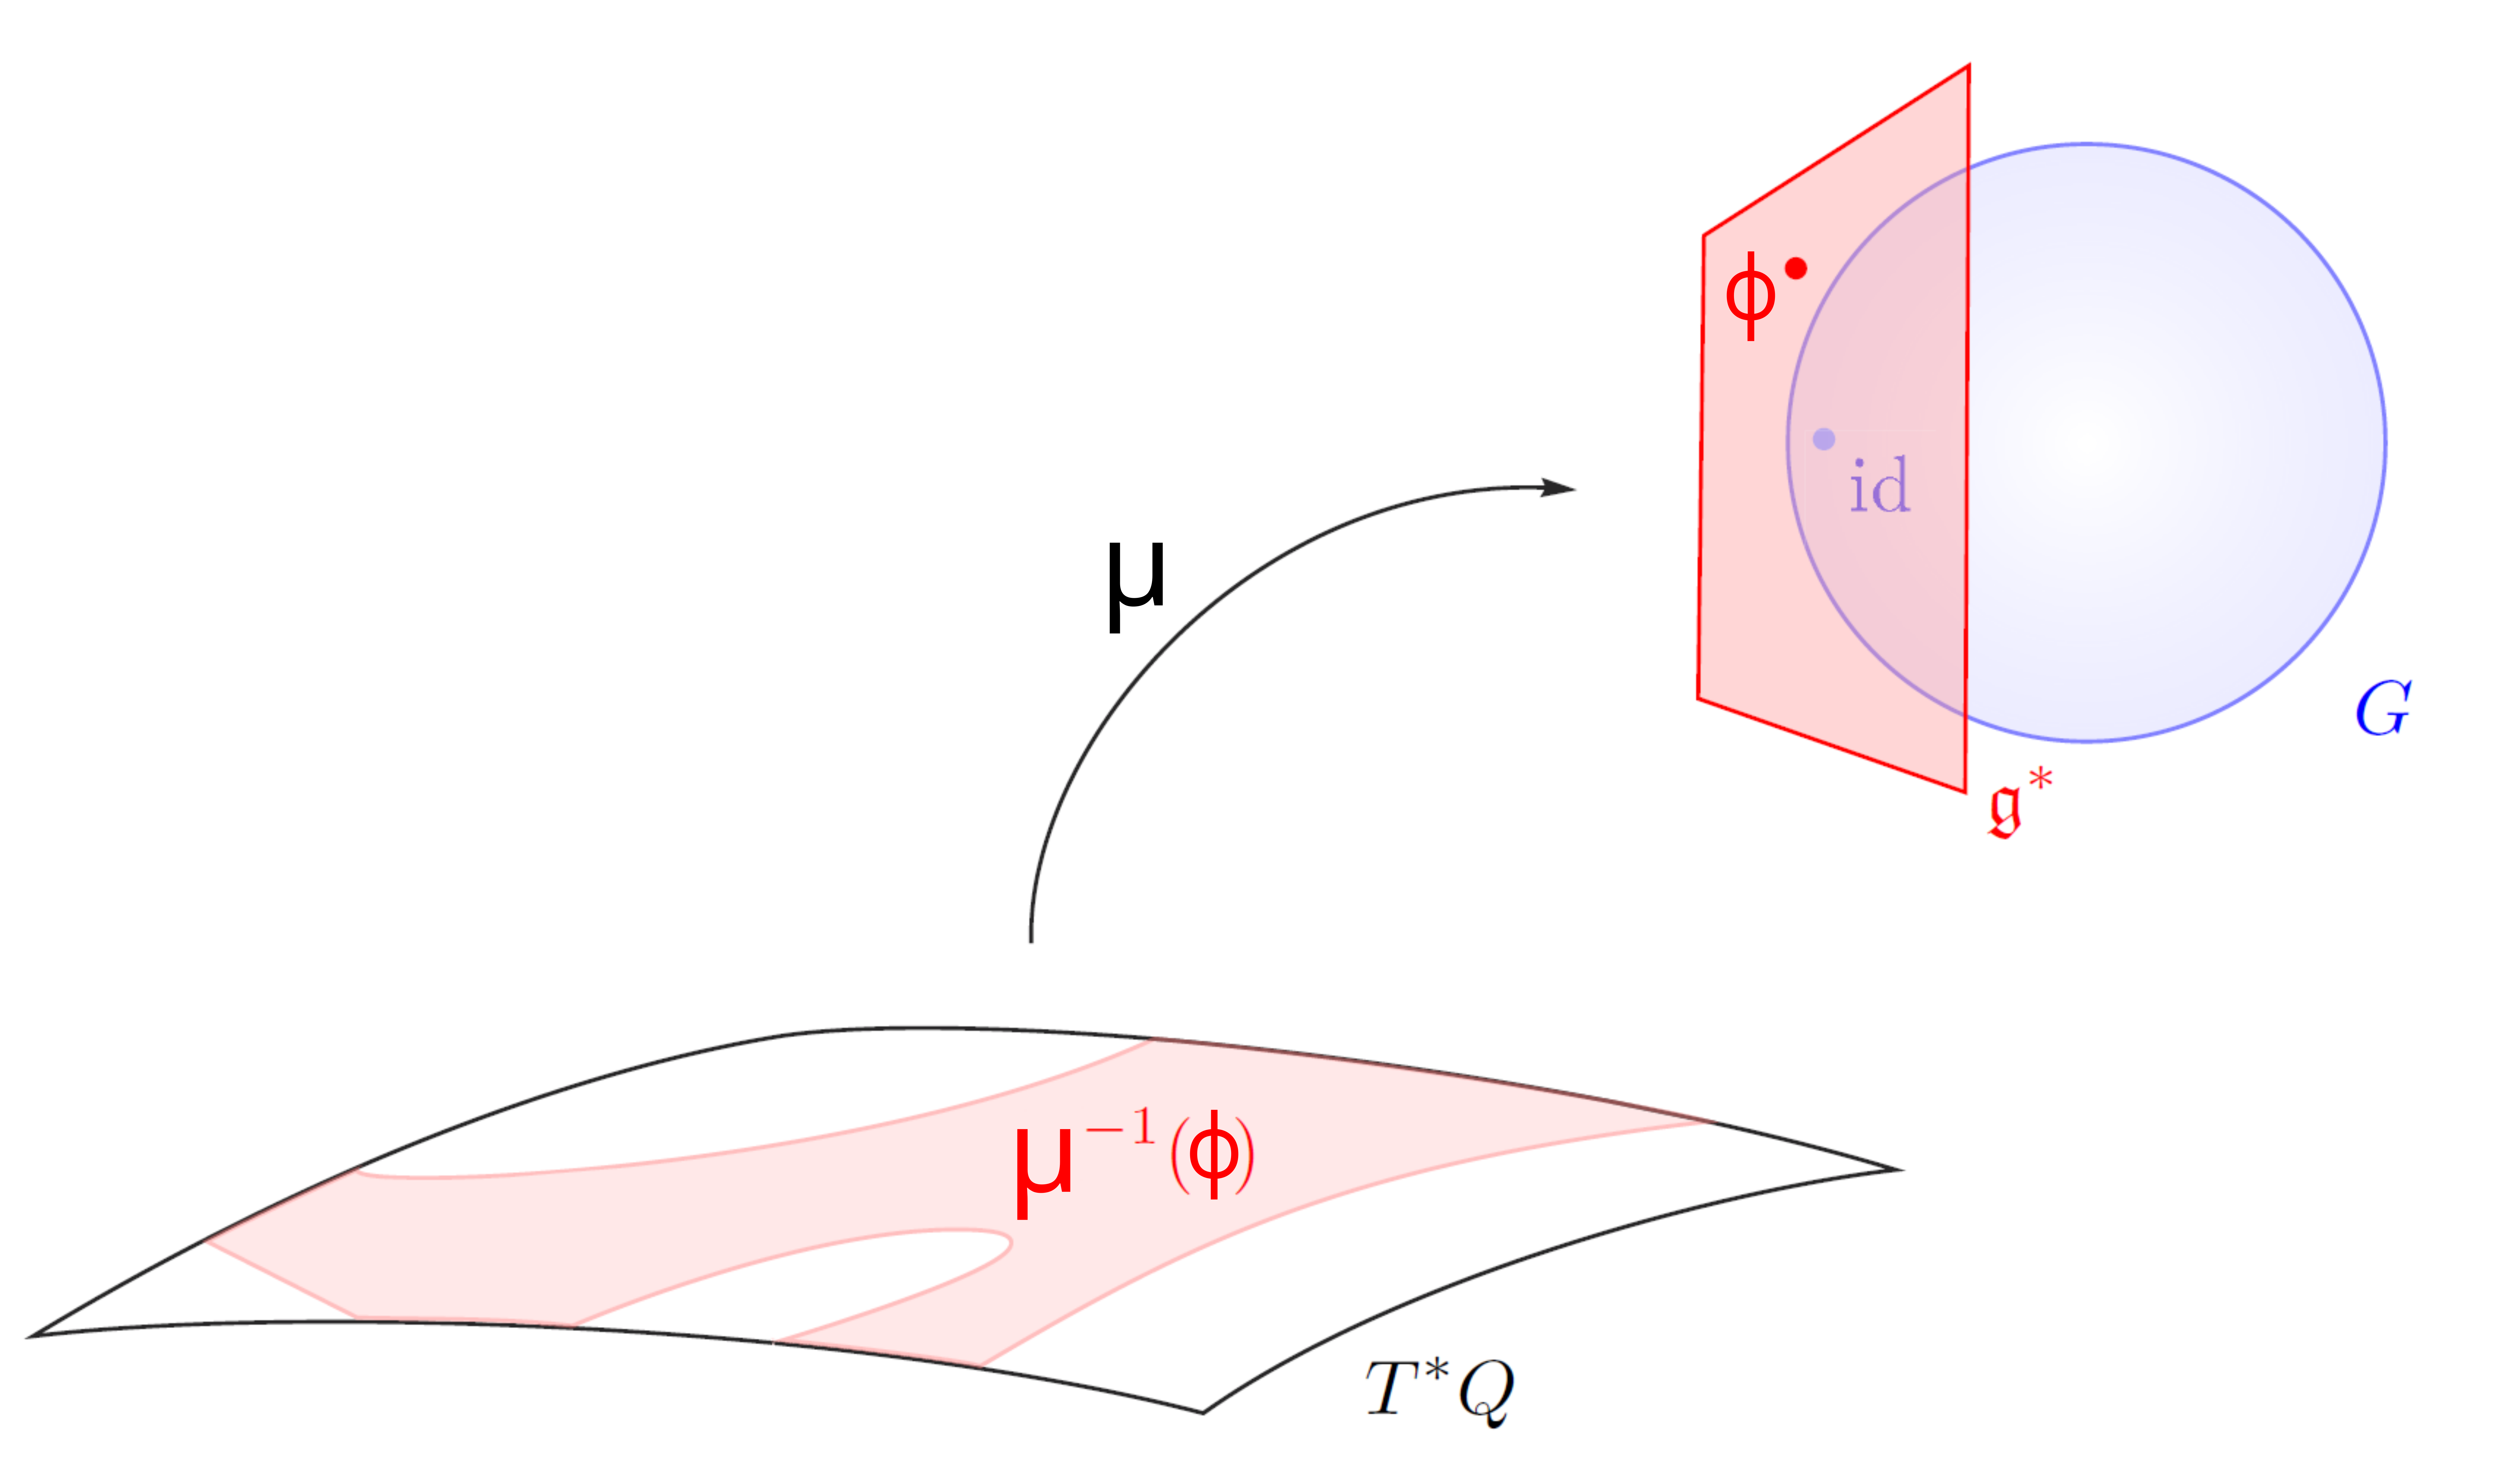
\includegraphics[width=.5\textwidth]{Pictures/Reduction}	
	\end{center}
	
	\textbf{\color{UniGreen}In mechanics:}~~
				\\
			{\it \small
				it embodies the process of restricting the dynamics of the system to the level sets of the conserved quantities pertaining to the symmetry group.		
			}
			\\[.2em]
			\color{gray}\small( e.g. restricting to studying a point-like particle in a central potential by studying it in radial coordinates)

\end{frame}
\note[itemize]{
	\item  \emph{(Credits to \href{https://math.gmu.edu/~cblacke/}{Casey Blacker} for the notes and to \href{https://arxiv.org/abs/1206.3302}{Christian Lessig} for the picture. See acknowledgements.}
	\item  In classical mechanics symmetry reduction plays an important role. Mathematically, this is usually phrased in terms of Marsden-Weinstein reduction
	\item {Symplectic Reduction} takes two inputs:
	\\ 1. Hamiltonian $G$-space $(M,\omega,{\color{orange}G},{\color{blue}\mu})$
	\\ 2. parameter ${\color{blue}\phi}\in\g^*$
	\item The \emph{reduced space} is $M_\phi:={\color{blue}\mu^{-1}(\phi)}{\color{orange}/G_\phi}$.
	\item (Marsden--Weinstein '74, Meyer '73) THM:\\
		If $\mu^{-1}(\phi)\subset M$ is smooth and $G_\phi\curvearrowright \mu^{-1}(\phi)$ is free and proper, then there is a \textbf{unique symplectic form} $\omega_\phi\in\Omega^2(M_\phi)$ such that $\pi^*\omega_\phi = i^*\omega$.



	\item Heuristic Approach to Reduction:
	\\1. describe $G\curvearrowright M$ in terms of $\omega$ 	\hspace{1cm}
	({\color{green}moment map $\mu$})
	\\2. identify a distinguished reduced space \hspace{1cm}
	({\color{green}reduction at $\mu=0$})
	\\3. use the ambiguity in 1.\ to obtain a family of reduced spaces \hspace{1cm}
	({\color{green}reduction at $\mu-\phi=0$, i.e.\ reduction at $\mu=\phi$}
	\\
	{\tiny Note: If $G_\phi\neq G$, then $\mu-\phi:M\to\g^*$ is not a moment map for either $G\curvearrowright M$ or $G_\phi\curvearrowright M$.}
	
}
%- . - . - . - . - . - . - . - . - . - . - . - . - . - . - . - . - . - . - . - . - . - . - . - .%	


 
%- . - . - . - . - . - . - . - . - . - . - . - . - . - . - . - . - . - . - . - . - . - . - . - .%
\begin{frame}[fragile]{Marsden-Weinstein-Meyer reduction}
	Consider: \quad $(M,\omega)$ symplectic,\quad $\theta:G\curvearrowright M$ $G$-action,\quad $\underline{\cdot}:\mathfrak{g}\to \mathfrak{X}(M)$ $\g$-action.
	\vfill\pause

	\begin{defblock}[Equivariant moment map]
		Smooth map $\quad\mu:M\to \mathfrak{g}^\ast\quad$ such that:
		
		\quad {\it i)} $\d\langle \mu,\xi\rangle = -\iota_{\underline{\xi}}\omega$,
		\qquad {\it ii)}  $\mu \circ \theta_g = Ad_g^\ast \circ \mu$,
		\qquad $\forall \xi \in \mathfrak{g},~ \forall g \in G$.
	\end{defblock}
	\vfill\pause

	\begin{thmblock}[Marsden-Weinstein reduction \cite{MarsdenWeinstein74}]
		\vspace{-.4em}\hspace{-1em}
		\begin{tabular}{l p{14cm}}
			Given: &   $\mu:M\to \mathfrak{g}^*$ equivariant moment map for $\color{orange}G\curvearrowright M$ $G$
			\\[.2em]
			Assume: & ${\color{blue}\phi} \in \mathfrak{g}^*$ regular value of $\mu$ 
			\qquad\quad \footnotesize \textcolor{gray}{($\Rightarrow$ $\mu^{-1}(\phi)\hookrightarrow M$ smooth embedding)}
			\\
			& $G_\phi\curvearrowright \mu^{-1}(\phi)$ free and proper
			\quad \footnotesize \textcolor{gray}{($\Rightarrow$ $\mu^{-1}(\phi)/G_\phi$ smooth manifold)}
			\\[.4em]
			Then: & \textbf{$\exists!$ symplectic structure} $\omega_\phi$ in $M_\phi:={\color{blue}\mu^{-1}(\phi)}{\color{orange}/G_\phi}$ \\
			& s.t. $\pi^\ast \omega_\phi = j^\ast \omega$ 
			\qquad {\footnotesize with $j:\mu^{-1}(\phi) \hookrightarrow M$ and $\pi:\mu^{-1}(\phi)\twoheadrightarrow M_\mu$}
		\end{tabular}
		\vspace{-.4em}
	\end{thmblock}
	%
	\vfill
	\begin{center}
	\begin{tikzpicture}[scale=2]
		\node[blue] (A) at (0,0) {$\mu^{-1}(\phi)$};
		\node[gray] (A1) at (0,.3) {$i^*\omega$};
		\node[gray] (A2) at (-.6,0) {$\pi^*\omega_\phi$};
		\node[blue] (B) at (1,0) {$M$};
		\node[gray] (B1) at (1,.3) {$\omega$};
		\node[orange] (C) at (0,-.8) {$M_\phi$};
		\node[gray] (C2) at (-.6,-.8) {$\omega_\phi$};

		\path[right hook->,blue] (A) edge node[above] {$i$} (B);
		\path[orange,->] (A) edge node[left] {$\pi$} (C);
		\begin{scope}[xshift=-1.8cm]
			\node[blue] at (0,0) {\small restrict to $\{\mu=\phi\}$};
			\node[orange] at (.15,-.4) {\small quotient by $G_\phi$};
		\end{scope}
	\end{tikzpicture}
	\end{center}


\end{frame}
\note[itemize]{
 \item 
	Let $(M,\omega)$ symplectic, $G\circlearrowright M$ be a Lie group action\pause and $\mu:M\to \mathfrak g^*$ such that: 
	\item  $\mu$ is a momentum, i.e. the infinitesimal action $\xi\mapsto \underline\xi:\mathfrak g\to \mathfrak X(M)$ of $G$ satisfies $X_{\langle\mu,\xi\rangle}=\underline \xi$. 
	\item $\mu$ is $G$-equivariant, i.e. $\mu(gm)=Ad^*_g\mu(m)$ 
	\item Then $\exists!$ symplectic form $\omega_r$ on $M_r=\frac{\mu^{-1}(0)}{G}$ such that $\pi^*\omega_r=i^*\omega$.
%% https://q.uiver.app/#q=WzAsMyxbMCwwLCJNIl0sWzMsMCwiXFxtdV57LTF9KDApIl0sWzYsMCwiTV9yIl0sWzEsMCwiaVxcXFwgXFxzdWJzdGFja3tpbmNsdXNpb25+b2Z+c3Vic3BhY2V9IiwyLHsic3R5bGUiOnsidGFpbCI6eyJuYW1lIjoiaG9vayIsInNpZGUiOiJib3R0b20ifX19XSxbMSwyLCJcXHBpXFxcXCBcXHN1YnN0YWNre3F1b3RpZW50fmJ5fnJlbGF0aW9ufSJdXQ==
%\[\begin{tikzcd}
%	M &&& {\mu^{-1}(0)} &&& {M_r}
%	\arrow["\begin{array}{c} i\\ \substack{inclusion~of~subspace} \end{array}"', hook', from=1-4, to=1-1]
%	\arrow["\begin{array}{c} \pi\\ \substack{quotient~by~relation} \end{array}", two heads, from=1-4, to=1-7]
%\end{tikzcd}\]
	\item 	The action of $G$ on $\mu^{-1}(0)$ is free and proper $\Rightarrow$ $0$ is reg. val. of $\mu$


}
%- . - . - . - . - . - . - . - . - . - . - . - . - . - . - . - . - . - . - . - . - . - . - . - .%


 


%- . - . - . - . - . - . - . - . - . - . - . - . - . - . - . - . - . - . - . - . - . - . - . - .%
\subsection{Singular reduction}
\begin{frame}{Symplectic singular reduction schemes}
	\begin{block}{The gist of singular reduction}
		 \begin{itemize}
			 \item[-] when $\mu$ is singular (i.e. $\mu^{-1}(0)$ is not a mfd.), the (geometrically) reduced space may not exist.
			 \item[-] a \emph{singular reduction scheme} is a procedure to construct a "reduced" algebra of observable out of the given data
			 \item[-] such that it corresponds to the algebra of observable of the reduced manifold in the regular case.
		 \end{itemize}
	\end{block}
	 %
	 \pause
	 \vfill
	 %
	\begin{thmblock}[Sniatycki-Weinstein reduction \cite{SniatyckiWeinstein83}]
		\vspace{-.4em}\hspace{-1em}
		\begin{tabular}{l p{14cm}}
			Given: & $(M,\omega)$ symplectic
			\\
			& $G\curvearrowright M$ symplectic with equivariant momap. $\mu:M\to \mathfrak{g}^*$
			\\[.4em]
			Then: & 
			$\displaystyle \left[\sfrac{C^\infty(M)}{I_\mu}\right]^G$
			admits a Poisson algebra structure 
			\footnote{$I_\mu$ = associative ideal generated by $\check{\mu}(\g)$ with $\check{\mu}(\xi):=\langle\mu,\xi\rangle$ the comomentum map.}			
			\\
			& it agrees with the M--W reduction in the regular case.		
		\end{tabular}
		\vspace{-.4em}
	\end{thmblock}
 \end{frame}
\note[itemize]{
 \item Let $(M,\omega,G,\mu)$ be a symplectic Hamiltonian $G$-space.
 \item The \emph{momentum ideal} is the associative ideal $I_\mu\subset C^\infty(M)$ generated by the momenta $\mu_{\xi}$ for any $\xi\in \mathfrak{g}$.
		Namely
		\[
			I_\mu 
			= 
			\Big\langle \mu_\xi \Big\rangle_{\xi \in \mathfrak{g}}^{\text{\tiny asso.}} 
			=
			\left\{
				\left.
					\sum_{i=1}^n f_i ~ \mu_{\xi_i}
				\right|~
					f_i \in C^\infty(M),~ \xi_i\in \mathfrak{g},~  1 \leq i \leq n
			\right\}
		\]

 \item The \emph{\'Sniatycki--Weinstein reduction} is the Poisson algebra
		\[
			\left(C^\infty(M)/I_\mu\right)^G.
		\]


}
%- . - . - . - . - . - . - . - . - . - . - . - . - . - . - . - . - . - . - . - . - . - . - . - .%	











%- . - . - . - . - . - . - . - . - . - . - . - . - . - . - . - . - . - . - . - . - . - . - . - .%
\subsection{Constraints Algebras}
\begin{frame}[fragile]{Attempting algebraic reduction naively}
When the action is not 'free and proper', we can try to mimic this directly using the function algebras:
% https://q.uiver.app/#q=WzAsNixbMCwwLCJNIl0sWzEsMCwiXFxtdV57LTF9KDApPVMiXSxbMywwLCJNX3IiXSxbMCwxLCJDXlxcaW5mdHkoTSkiXSxbMSwxLCJDXntcXGluZnR5fShTKT1cXGZyYWN7Q157XFxpbmZ0eX0oTSl9e0lfe1N9fSJdLFszLDEsIkNee1xcaW5mdHl9KE1fcik9Q15cXGluZnR5KFMpXkciXSxbMSwyLCJcXHN1YnN0YWNre3F1b3RpZW50fSIsMCx7InN0eWxlIjp7ImhlYWQiOnsibmFtZSI6ImVwaSJ9fX1dLFszLDQsIlxcc3Vic3RhY2t7cXVvdGllbnR9IiwwLHsic3R5bGUiOnsiaGVhZCI6eyJuYW1lIjoiZXBpIn19fV0sWzAsMSwiXFxzdWJzdGFja3tyZXN0cmljdGlvbn0iLDAseyJzdHlsZSI6eyJib2R5Ijp7Im5hbWUiOiJzcXVpZ2dseSJ9fX1dLFs0LDUsIlxcc3Vic3RhY2t7cmVzdHJpY3Rpb259IiwwLHsic3R5bGUiOnsiYm9keSI6eyJuYW1lIjoic3F1aWdnbHkifX19XV0=
\[\begin{tikzcd}
	M & {\mu^{-1}(0)=S} && {M_r} \\
	{C^\infty(M)} & {C^{\infty}(S):=\frac{C^{\infty}(M)}{I_{S}}} && {C^{\infty}(M_r)=C^\infty(S)^G}
	\arrow["{\substack{restriction}}", squiggly, from=1-1, to=1-2]
	\arrow["{\substack{quotient}}", two heads, from=1-2, to=1-4]
	\arrow["{\substack{quotient}}", two heads, from=2-1, to=2-2]
	\arrow["{\substack{restriction}}", squiggly, from=2-2, to=2-4]
\end{tikzcd}\]

where $I_S=\{f\in C^{\infty}(M)~|~f|_S=0\}$.
\pause 
\vfill
Equivalently:

% https://q.uiver.app/#q=WzAsMyxbMCwwLCJDXlxcaW5mdHkoTSkiXSxbMiwwLCJOX1M9XFx7Zn58fiBmXFxpbiBDXlxcaW5mdHkoTSl8X1N+fkdcXG1hdGhybXstaW52YXJpYW50fVxcfSJdLFs0LDAsIlxcZnJhY3tOX1N9e0lfU30iXSxbMCwxLCJcXHN1YnN0YWNre3Jlc3RyaWN0aW9ufSIsMCx7InN0eWxlIjp7ImJvZHkiOnsibmFtZSI6InNxdWlnZ2x5In19fV0sWzEsMiwiXFxzdWJzdGFja3txdW90aWVudH0iLDAseyJzdHlsZSI6eyJoZWFkIjp7Im5hbWUiOiJlcGkifX19XV0=
\[\small\begin{tikzcd}
	{C^\infty(M)} && {N_S=\{f~|~ f\in C^\infty(M)|_S~~G\mathrm{-invariant}\}} && {\frac{N_S}{I_S}}
	\arrow["{\substack{restriction}}", squiggly, from=1-1, to=1-3]
	\arrow["{\substack{quotient}}", two heads, from=1-3, to=1-5]
\end{tikzcd}\]
\pause
\vfill

\begin{alertblock}{Problem}
	$C^\infty(S)^G=\frac{N_S}{I_S}$ is not a Poisson algebra in general.
\end{alertblock}
(when constraints not first class, cf. Dirac reduction)
\end{frame}
\note[itemize]{
	\item \emph{(Credits to \href{https://www.ryvkin.eu/}{Leonid Ryvkin} for the tex code of this slide.)}
}
%- . - . - . - . - . - . - . - . - . - . - . - . - . - . - . - . - . - . - . - . - . - . - . - .%



%- . - . - . - . - . - . - . - . - . - . - . - . - . - . - . - . - . - . - . - . - . - . - . - .%
\begin{frame}{Constraint Algebras} 
	\begin{block}{Idea:}
	    \begin{itemize}[noitemsep,topsep=0pt,parsep=0pt,partopsep=0pt]
			\item[-] Both regular/geometric and singular/algebraic reduction are 2-steps procedures (1. restrict 2. quotient).
			\item[-] Let's work in a category where all data needed for the reduction are bundled together in a suitable categorical objects. {\tiny (To avoid pathologies arising from these steps)}
	    \end{itemize}
	\end{block}
	\pause
	\vfill
	\begin{defblock}[Constraint algebra triples \cite{Dippell2023}]
		A (strong embedded) constraint algebra $\mathcal A$ is given by a triple $(\mathcal A_T, \mathcal A_N, \mathcal A_0)$, where
		\begin{itemize}[noitemsep,topsep=0pt,parsep=0pt,partopsep=0pt]
			\item[•] $\mathcal A_T$ is an algebra \emph{("total space")}
			\item[•] $\mathcal A_N\subset \mathcal A_T$ a subalgebra  \emph{("normal space")}
			\item[•] $\mathcal A_0\subset \mathcal A_N$ a two-sided ideal in $\mathcal A_T$ \emph{("zero space")}
		\end{itemize}
	\end{defblock}
	\vfill
	\pause
	\begin{exblock}
		Let $S$ be a closed set. Algebraically, we describe $C^\infty(S)$ by $\frac{C^\infty(M)}{I_S}$.
		\\ 
		We can think of it as the constraint triple:
		$$
			\mathcal A=(\mathcal A_T,\mathcal A_N,\mathcal A_0)=(C^\infty(M),C^\infty(M), I_S)
		$$
	\end{exblock}

\end{frame}
\note[itemize]{
	\item  triples of the type (algebra , subalgebra, ideal).
	\item After \cite{Dippell2023} we call such triples { \bf constraint triples} and their parts \emph{total space, normal space, zero space}.
	\item It is a (strong) constraint algebra if $\mathcal A_0\subset \mathcal A_N\subset \mathcal A_T$ subalgebras and $\mathcal A_0\subset \mathcal A_T$ ideal.
}
%- . - . - . - . - . - . - . - . - . - . - . - . - . - . - . - . - . - . - . - . - . - . - . - .%


%- . - . - . - . - . - . - . - . - . - . - . - . - . - . - . - . - . - . - . - . - . - . - . - .%
\begin{frame}{A plethora of approaches to singular reduction}
 	Many singular reduction schemes adhere to this pattern!
 	\vfill
 	\pause
\begin{table}[]
	\begin{tabular}{l|l|l||l}
		algebra $\mathcal{A}_T$ & subalgebra $\mathcal{A}_N$ & ideal $\mathcal{A}_0$ & comment \\
		\hline
		
		$C^\infty(M)$&      $N_S$     &   $I_S$   &  $\substack{S=\mu^{-1}(0),~ I_S=\{f~|~f|_S=0\}}$ \\
			&&&  $\substack{N_S= \{ f | gf-f\in I_S \forall g\in G\}}$ \\
	& & & \color{red} not Poisson \\ 
	\hline	\pause
	$C^\infty(M)$&   $F_S$         &   $I_S$   &  $\substack{F_S=\{f~|~\{f,I_S\}\subset I_S\}}$ \\
	& & & \color{red} if $I_S\subset F_S$\\
	\hline \pause
	
	$C^\infty(M)$&   $C^\infty(M)^G$         &   $(I_S)^G$   &  $\substack{C^\infty(M)^G=\{f~|~gf=f\forall g\in G\}}$ \\
	\hline \pause
		$C^\infty(M)$&   $C^\infty(M)^G$         &   $(I_\mu)^G$   & $\substack{I_\mu=\{\sum_{i=1}^k f_i\langle \mu,\xi_i\rangle|~f_i\in C^\infty(M), \xi_i\in \mathfrak g\}}$\\
		\hline \pause
	$C^\infty(M)$&      $N_\mu$     &   $I_\mu$   & $\substack{N_\mu= \{ f | gf-f\in I_\mu \forall g\in G\}}$ \footnote{When $G$ connected $N_\mu=N(I_\mu):=\{f~|~\{f,I_\mu\}\subset I_\mu\}$.}\\
	\hline 
		
	\end{tabular}\pause
\end{table}
	\vfill
	{\bf Remarks }names in order: 'naive' , Dirac, Sniatycki, Arms-Cushman-Gotay, Sniatycki-Weinstein.

\end{frame}
\note[itemize]{
	\item \emph{(Credits to \href{https://www.ryvkin.eu/}{Leonid Ryvkin} for the tex code of this slide.)}
}
%- . - . - . - . - . - . - . - . - . - . - . - . - . - . - . - . - . - . - . - . - . - . - . - .%


%- . - . - . - . - . - . - . - . - . - . - . - . - . - . - . - . - . - . - . - . - . - . - . - .%
\begin{frame}{Constraint Gerstenhaber-Modules}

%
\begin{defblock}[Constraint Gerstenhaber algebra {(\cite[Def. 2.25]{dippelkern})}]
	A constraint algebra $G=\triple{G}$ equipped with a constraint bilinear map
	\begin{displaymath}
		\{ \cdot, \cdot \} \colon G[1] \otimes G[1] \to G[1]
	\end{displaymath}
	such that $G_\Total$ is a Gerstenhaber algebra. 
\end{defblock}
\pause\vfill
%

 \begin{remblock}[$G$ can be seen as a triple of Gerstenhaber subalgebras]\label{rk:constraintgerst-as-triple}
	 $G_\Null \subseteq G_\Wobs \subseteq (G_\Total, \wedge,\lbrace\cdot,\cdot\rbrace)$ such that $G_\Null$ is a Gerstenhaber ideal in $G_\Wobs$. 
\end{remblock}
\pause\vfill
%

\begin{defblock}[Constraint Gerstenhaber module]\label{def:constraintgerstmodule}
	A constraint vector space $V=\triple{V}$ endowed with a constraint Gerstenhaber algebra structure on the space $G \oplus V^\rev$ such that the multiplication and the bracket are trivial when restricted to $V^\rev$.
\end{defblock}
\vfill

\end{frame}
\note[itemize]{
	\item  We have seen how the notion of BV-modules can be understood as a Cartan calculus. In this section, we will adapt this notion to the setting of constraint algebras and modules.
	\item Details: constraint morphisms, tensor products, strongness.
	\item the following four equations hold:
	%
	\begin{align*}
		\{ G_\Wobs, G_\Wobs \} &\subseteq G_\Wobs~,&& G_\Wobs \wedge G_\Wobs \subseteq G_\Wobs~, \\
		\{ G_\Null, G_\Wobs \} &\subseteq G_\Null~,&& G_\Wobs \wedge G_\Null \subseteq G_\Null ~.
	\end{align*}
	For a strong Gerstenhaber algebra, we would also need to check $G_\Null \wedge G_\Total \subseteq G_\Null$ as the only additional condition.
	\item Since every constraint Gerstenhaber algebra is, in particular, a graded constraint algebra and a graded constraint Lie algebra, we know that ${G}_{\red}$ carries the structures of a graded algebra and a graded Lie algebra. Moreover, it is easy to see that the graded Leibniz rule on ${G}$
induces a graded Leibniz rule on ${G}_{\red}$, showing that ${G}_{\red}$ forms itself a Gerstenhaber algebra.
	\item An \emph{(embedded, $\mathbb Z$-graded) constraint vector space} $V$ is given by a triple $V=(V_\Total,V_\Wobs,V_\Null)$, where $V_\Total$ is a $\mathbb Z$-graded vector space and $V_\Null\subset V_\Wobs\subset V_\Total$ are subspaces. A \emph{morphism} $f:V\to V'$ of constraint vector spaces is a linear map $f:V_\Total\to V'_\Total$ such that $f(V_\Wobs)\subset V'_\Wobs$ and $f(V_\Null)\subset V'_\Null$.
}
%- . - . - . - . - . - . - . - . - . - . - . - . - . - . - . - . - . - . - . - . - . - . - . - .%
 

%- . - . - . - . - . - . - . - . - . - . - . - . - . - . - . - . - . - . - . - . - . - . - . - .%
\begin{frame}{Constraint Cartan calculus}
%
\begin{defblock}[Constraint BV-module]\label{def:constraintbv}
	A Gerstenhaber module $V=\triple{V}$ endowed with a constraint degree $1$ homomorphism
	$$
		\d \colon V \to V[1]~,
	$$
	such that $(V_\Total, \d_\Total)$ is a BV-module over $G_\Total$.
\end{defblock}
\pause\vfill
%

\begin{remblock}[Constraint Cartan calculus]
	The con. BV-module structure implies the existence of constraint morphisms
	$$ \iota: G\otimes V^{\rev} \to V^{\rev}, \d: V \to V[1] \text{ and } \Lie: G\otimes V^{\rev} \to V^{\rev}[-1] $$ satisfying six commutation rules as before.
\end{remblock}
\vfill

\end{frame}
\note[itemize]{
	\item 
}
%- . - . - . - . - . - . - . - . - . - . - . - . - . - . - . - . - . - . - . - . - . - . - . - .%

%- . - . - . - . - . - . - . - . - . - . - . - . - . - . - . - . - . - . - . - . - . - . - . - .%
\begin{frame}[shrink]{Constraint $L_\infty$ Algebra Associated with a constraint BV-module}
	%
	\begin{defblock}[Constraint $L_\infty$-algebras] 
	A constraint vector space $L=\triple{L}$  equipped with \\
	a collection of constraint multilinear maps $l_j \colon L^{\otimes j} \to L[2-j]$\\
	such that $(L_\Total, (l_j)_\Total)$ is an $L_\infty$-algebra.
	\end{defblock}
	\pause\vfill
	%
	
	Let $V$ a cons. BV-module over a cons. Gerst. algebra $G$,  $\omega\in V_\Wobs^{k+1}$ a cocycle.
	\begin{defblock}[Constraint vector space of Hamiltonian pairs]\label{def:constraint-algebraicham0}
		The	 \emph{constraint ungraded vector space}:
		$$
		\Ham^0(V, \omega) := 
		\colvec{
			\big\{ (\alpha, X) \in V^{k-1}_\Total \oplus G_\Total^1 \mid \iota_X \omega = -\d\alpha \big\}
			\\
			\Ham^0(V, \omega) \cap \big(V_\Wobs \oplus G_\Wobs\big)
			\\
			\Ham^0(V, \omega) \cap \big( V_\Null \oplus G_\Null \big)
		}
		~.
		$$
	\end{defblock}
	\pause\vfill
	%

	\begin{defthmblock}[Constraint $L_\infty$-algebra of observables]
		The \emph{constraint $\Z$-graded vector space}
  		$$
  		\Ham(V, \omega)^i := 
		\begin{cases}
    		V^{k-1 + i} & i \leq -1, \\
    		\Ham^0(V, \omega) & i = 0,\\
    		0 & i \geq 1~;
  		\end{cases} 
  		$$
	endowed with the family of cons. multilinear maps \( l_j \colon \Ham^{\otimes j}(V, \omega) \to \Ham(V, \omega)[2-j] \) defined via cons. multicontractions with $\omega$.
	\end{defthmblock}
 
	
\end{frame}
\note[itemize]{
	\item  Building on the chosen embedded constraint setting, one can further define constraint $L_\infty$-algebras in close analogy with the classical case.
	\item 	Since we work in the embedded setting, a constraint $L_\infty$-algebra $L$ as per \autoref{def:constraintlinfty} is given by a sequence of $L_\infty$-subalgebras $L_\Null \subseteq L_\Wobs \subseteq (L_\Total,(l_j)_\Total)$ such that $L_\Null$ is in particular an $L_\infty$-ideal  in $L_\Wobs$ in the following sense:
	\begin{displaymath}
		l_j\big(L_\Null, L_\Wobs,\dots, L_\Wobs\big)
		\subseteq L_\Null~, \quad \forall j \geq 1~.
	\end{displaymath}
	Therefore, is assured that the $L_\infty$-algebra structure on $L_\Total$ induces a well-defined $L_\infty$-algebra structure on the reduced space $\red(L) := L_\Wobs / L_\Null$ (compare with \autoref{rk:constraintalgebras-as-triples}).
	\item 	The space of Hamiltonian pairs can be interpreted as the fibered product \( V^{k-1} \times_{V^k} G^1 \) in the category of constraint vector spaces. 
	This perspective yields, in particular, three pullback diagrams, one for each component of the constraint vector space described.
}
%- . - . - . - . - . - . - . - . - . - . - . - . - . - . - . - . - . - . - . - . - . - . - . - .%


%- . - . - . - . - . - . - . - . - . - . - . - . - . - . - . - . - . - . - . - . - . - . - . - .%
\begin{frame}{Reduction Functor}

	\begin{remblock}[Reduction functor]\label{rk:red-functor}
		The very purpose of introducing categories of constraint objects is to assume the existence of a corresponding \emph{reduction functor} $\red$ that assigns to each constraint object its reduced counterpart.
	\end{remblock}
	\vfill\pause

	\begin{exblock}[Constraint associative algebras]
	A constraint associative algebra is equivalently given by a triple $A = \triple{A}$, where $A_\Wobs \subset A_\Total$ is a subalgebra, and $A_\Null \subset A_\Wobs$ is a (two-sided) ideal. i.e.:
		$$
			\red: \textbf{ConAlg} \to \textbf{Alg}~, \quad \mathcal A \mapsto \red(\mathcal A) := \mathcal A_\Wobs / \mathcal A_\Null~,
		$$
	\end{exblock}
	\vfill\pause

	\begin{upshotblocktitle}[Reduction functor for the $L_\infty$-algebra of observables]
		The $\Null$ part of $\Ham(V, \omega)$ is an $L_\infty$-ideal in the $\Wobs$ part. 
		\\
		Thus, the reduction functor applied to the constraint $L_\infty$-algebra of observables space gives a honest $L_\infty$-algebra.
	\end{upshotblocktitle}

\end{frame}
\note[itemize]{
	\item  	The reduction functor $\red$ assigns to each object $V$ the quotient vector space $\red(V) := V_\Wobs/V_\Null$, and to each morphism $f: V \to V'$ the induced map $\red(f): V_\Wobs/V_\Null \to V'_\Wobs/V'_\Null$.

}
%- . - . - . - . - . - . - . - . - . - . - . - . - . - . - . - . - . - . - . - . - . - . - . - .%


%-----------------------------------------------------------%
\ifstandalone
% https://en.wikibooks.org/wiki/LaTeX/Bibliographies_with_biblatex_and_biber
\begin{frame}[t,allowframebreaks]{Bibliography}
	%\nocite{*}
	\printbibliography
\end{frame}
\fi
%-----------------------------------------------------------%



%-----------------------------------------------------------+
\end{document}
%-----------------------------------------------------------+



%-----------------------------------------------------------%



%--------------------------------------------------------------------------------------------------%
	\addtocounter{framenumber}{-1}
		\begin{frame}{Conclusion:}
			\vfill
		  \centering 
		  \onslide<2->{\Huge\color{red} 
		  \emph{Thank you for your attention!}\normalsize \color{black}}
			\vfill
			%
 
		\end{frame}
		\note[itemize]{
			\item
		}
%------------------------------------------------------------------------------------------------



%------------------------------------------------------------------------------------------------
% APPENDIX
%------------------------------------------------------------------------------------------------
\appendix
%------------------------------------------------------------------------------------------------
\section{Complementary Material}
	%%- HandOut Flag ----------------------
\makeatletter
\@ifundefined{ifHandout}{%
  \expandafter\newif\csname ifHandout\endcsname
}{}
\makeatother

%- D0cum3nt ----------------------------------------------------------------------------------------------
%\documentclass[beamer,10pt]{standalone}   
\documentclass[beamer,10pt,handout]{standalone}  \Handouttrue  

\ifHandout
	\setbeameroption{show notes} %print notes   
\fi

	
%- Packages ----------------------------------------------------------------------------------------------
\usepackage{custom-style}
\usepackage{math}



%--Beamer Style-----------------------------------------------------------------------------------------------
\usetheme{toninus}
\usepackage{animate}
\usetikzlibrary{positioning, arrows}
\usetikzlibrary{shapes}


%- Bibliography (Biber) ----------------------------------------------------------------------------------
\usepackage[backend=biber,style=alphabetic,maxnames=2]{biblatex}
\bibliography{bibfile.bib}

%===========================================================%
\begin{document}
%===========================================================%
\checkpoint

%- . - . - . - . - . - . - . - . - . - . - . - . - . - . - . - . - . - . - . - . - . - . - . - .%	
\subsection{Reduction} 
%- . - . - . - . - . - . - . - . - . - . - . - . - . - . - . - . - . - . - . - . - . - . - . - .%	

%- . - . - . - . - . - . - . - . - . - . - . - . - . - . - . - . - . - . - . - . - . - . - . - .%
\begin{frame}{Reminder: momentum maps in symplectic geometry}\label{frame:symplecticmomaps}
	Consider $\theta:G\curvearrowright M$ symplectic,~~ $\underline{\cdot}:\mathfrak{g}\to \mathfrak{X}(M)$ infinitesimal action.
	\vfill

	\begin{columns}[T]
		\setlength{\belowdisplayskip}{5pt}
		\begin{column}{.50\linewidth}
			%
			\centering \it
			\onslide<2->{
				\begin{defblock}[Equivariant moment map]
					Smooth map $$\mu:M\to \mathfrak{g}^\ast$$
					such that:
					\begin{itemize}
						\item[i.] $d\langle \mu,\xi\rangle = -\iota_{\underline{\xi}}\omega$ 
						~\qquad, $\forall \xi \in \mathfrak{g}$
						\item[ii.] $\mu \circ \theta_g = Ad_g^\ast \circ \mu$
						 \qquad\small, $\forall g \in G$
					\end{itemize}
				\end{defblock}
			}
		\end{column}	
		%
		\onslide<2->{\vrule{}}
		%
		\begin{column}{.50\linewidth}
			\onslide<3->{			
				\begin{defblock}[Comoment map]
					Linear map $$\widetilde{\mu}: \mathfrak{g}\to C^\infty(M,\omega)$$
					such that:
					\begin{itemize}
						\item[i.] $d\widetilde{\mu}(\xi) = -\iota_{\underline{\xi}}\omega$ 
						\qquad~\small, $\forall \xi \in \mathfrak{g}$
						\item[ii.] $\widetilde{\mu}([\xi,\eta]) = \lbrace\widetilde{\mu}(\xi),\widetilde{\mu}(\eta)\rbrace$ \small, $\forall \xi,\eta \in \mathfrak{g}$
					\end{itemize}
				\end{defblock}
			}
		\end{column}	
	\end{columns}	
	%
	\pause
	\vspace{1em}
	%
	\begin{columns}[]
		\setlength{\belowdisplayskip}{5pt}
		\begin{column}{.40\linewidth}
			%
			\centering \it
			\onslide<5->{
				\begin{upshotblocktitle}[Duality]
					\begin{displaymath}
						\mu(x) : \mathfrak{\xi} \mapsto \widetilde{\mu}(\xi)\big\vert_x
					\end{displaymath}
					%
					\emph{
					\small
					"duality wrt. the currying operation"					
					}
				\end{upshotblocktitle}
			}
		\end{column}	
		%
		%
		\begin{column}{.60\linewidth}
			\onslide<4->{			
				\begin{upshotblocktitle}[$\widetilde{\mu}$ as a lift]
					\begin{displaymath}
						\begin{tikzcd}[ampersand replacement = \&]
						 \& C^\infty(M,\omega) \ar[d,"\vHam"]
						 \\
						 \mathfrak{g} \ar[ur,dashed,sloped,"\widetilde{\mu}"]\ar[r,"\underline{\cdot}"'] \& \mathfrak{X}(M)
						\end{tikzcd}
					\end{displaymath}
					%
					\emph{
					\small
					"it is a lift (in the Lie category) of the infinitesimal action by the assigment of hamiltonian v.fields."					
					}
				\end{upshotblocktitle}
			}
		\end{column}	
	\end{columns}		
\end{frame}
\note[itemize]{
		\item Moment maps are instrumental to the proper formalization of reduction in symplectic geometry.
		\item consider an action preserving the symplectic form.
		\item[-] $\langle \cdot, \cdot \rangle$ is the natural pairing of $\mathfrak{g}$ and $\mathfrak{g}^\ast$.
			\item[-] $\theta_g$ is the diffeomorphism associated to $g\in G$ via $\theta:G\curvearrowright M$
			\item[-] $Ad^\ast_g$ is the coadjoint action $G\curvearrowright \mathfrak{g}^\ast$
		\item The moment map can be reexpressed as a comomentum map.
		\item Observe that ii. on the left always implies ii. on the right. The converse is trure only if $G$ is connected.
		\item $G\curvearrowright M$ is said "Hamiltonian" (see slide \ref{frame:gisthamaction} in appendix) iff $\exists$ comoment map $\widetilde{\mu}$.
		\item \emph{moment map: Describe ${\color{orange}G\curvearrowright M}$ in terms of $\color{blue}C^\infty(M)\to\X(M)$.}
		\begin{center}
		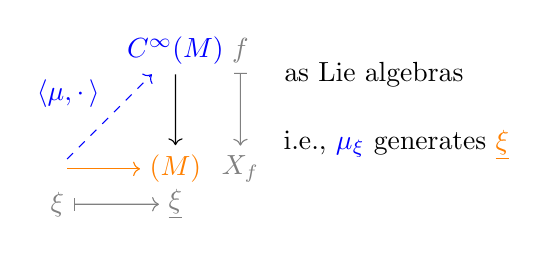
\begin{tikzpicture}[scale=1.5]
			\node[orange] (A) at (0,0) {$\g$};
			\node[gray] (A1) at (0,-.3) {$\xi$};
			\node[blue] (B) at (1,1) {$C^\infty(M)$};
			\node[gray] (B2) at (1.55,1) {$f$};
			\node[orange] (C) at (1,0) {$\X(M)$};
			\node[gray] (C1) at (1,-.3) {$\underline\xi$};
			\node[gray] (C2) at (1.55,0) {$X_f$};
	
			\path[->,blue,dashed] (A) edge node[above left] {$\langle\mu,\cdot\,\rangle$} (B);
			\path[->,orange] (A) edge (C);
			\path[->] (B) edge (C);
			\path[|->,gray] (A1) edge (C1);
			\path[|->,gray] (B2) edge (C2);
	
			\begin{scope}[xshift=3cm]
				\node at (-.32,.8) {as Lie algebras};
				\node at (-.13,.2) {i.e., {\color{blue}$\mu_\xi$} generates {\color{orange}$\underline\xi$}};
			\end{scope}
		\end{tikzpicture}
		
			\footnotesize		(\emph{moment map:} ${\color{blue}\mu:M\to\g^*}$, 
		 \emph{Hamiltonian $G$-space:} 	$(M,\omega,G,\mu)$)
		\end{center}
		\item
		 $\alpha\mapsto X_\alpha$ is a homomorphism of Leibniz algebras:
		$$\d\{\alpha,\beta\} = \d\L_{X_\alpha}\beta = \L_{X_\alpha}\iota_{X_\beta}\omega = \iota_{[X_\alpha,X_\beta]}\omega ~{\color{black!80} \implies}~
		X_{\{\alpha,\beta\}} = [X_\alpha,X_\beta]$$
}
%- . - . - . - . - . - . - . - . - . - . - . - . - . - . - . - . - . - . - . - . - . - . - . - .%



%- . - . - . - . - . - . - . - . - . - . - . - . - . - . - . - . - . - . - . - . - . - . - . - .%
\begin{frame}{Other approaches to singular reduction}
 	Many singular reduction schemes adhere to this pattern!
 	\vfill
 	\pause
\begin{table}[]
	\begin{tabular}{l|l|l||l}
		algebra $\mathcal{A}_T$ & subalgebra $\mathcal{A}_N$ & ideal $\mathcal{A}_0$ & comment \\
		\hline
		
		$C^\infty(M)$&      $N_S$     &   $I_S$   &  $\substack{S=\mu^{-1}(0),~ I_S=\{f~|~f|_S=0\}}$ \\
			&&&  $\substack{N_S= \{ f | gf-f\in I_S \forall g\in G\}}$ \\
	& & & \color{red} not Poisson \\ 
	\hline	\pause
	$C^\infty(M)$&   $F_S$         &   $I_S$   &  $\substack{F_S=\{f~|~\{f,I_S\}\subset I_S\}}$ \\
	& & & \color{red} if $I_S\subset F_S$\\
	\hline \pause
	
	$C^\infty(M)$&   $C^\infty(M)^G$         &   $(I_S)^G$   &  $\substack{C^\infty(M)^G=\{f~|~gf=f\forall g\in G\}}$ \\
	\hline \pause
		$C^\infty(M)$&   $C^\infty(M)^G$         &   $(I_\mu)^G$   & $\substack{I_\mu=\{\sum_{i=1}^k f_i\langle \mu,\xi_i\rangle|~f_i\in C^\infty(M), \xi_i\in \mathfrak g\}}$\\
		\hline \pause
	$C^\infty(M)$&      $N_\mu$     &   $I_\mu$   & $\substack{N_\mu= \{ f | gf-f\in I_\mu \forall g\in G\}}$ \footnote{When $G$ connected $N_\mu=N(I_\mu):=\{f~|~\{f,I_\mu\}\subset I_\mu\}$.}\\
	\hline 
		
	\end{tabular}\pause
\end{table}
	\vfill
	{\bf Remarks }names in order: 'naive' , Dirac, Sniatycki, Arms-Cushman-Gotay, Sniatycki-Weinstein.

\end{frame}
\note[itemize]{
	\item \emph{(Credits to \href{https://www.ryvkin.eu/}{Leonid Ryvkin} for the tex code of this slide.)}
}
%- . - . - . - . - . - . - . - . - . - . - . - . - . - . - . - . - . - . - . - . - . - . - . - .%
 



%-----------------------------------------------------------%
\ifstandalone
% https://en.wikibooks.org/wiki/LaTeX/Bibliographies_with_biblatex_and_biber
\begin{frame}[t,allowframebreaks]{Bibliography}
	%\nocite{*}
	\printbibliography
\end{frame}
\fi
%-----------------------------------------------------------%



%-----------------------------------------------------------+
\end{document}
%-----------------------------------------------------------+



	%\input{bv-triples-aknowledgements}
%------------------------------------------------------------------------------------------------

%+----------------------------------------------------------+
\end{document}
%+----------------------------------------------------------+
 
 
